\documentclass[twoside]{ctuthesis}

\ctusetup{
	mainlanguage = english,
	title-czech = {Simulace hloubkových senzorů pro autonomní učení a testování},
	title-english = {Simulating depth measuring sensors for autonomous learning and benchmarking},
	xdoctype = M,
	doctype-english = {Master thesis},
	xfaculty = F3,
	department-czech = {Katedra Kybernetiky},
	department-english = {Department of Cybernetics},
	author = {Otakar Jašek},
	supervisor = {doc. Ing. Karel Zimmermann, PhD.},
%	keywords-czech = {Faster \rcnn{}, Konvoluční neuronové sítě, přetrénování neuronových sítí, detekce a rozpoznání objektu},
%	keywords-english = {Faster \rcnn{}, Convolutional neural networks, fine-tuning of neural networks, detection and recognition of objects},
	fieldofstudy-english = {Open Informatics},
	subfieldofstudy-english = {Computer Vision and Digital Image},
	fieldofstudy-czech = {Otevřená Informatika},
	subfieldofstudy-czech = {Počítačové vidění a digitální obraz},
	specification-file = zadani.pdf,
	front-specification = true,
	day = 25,
	month = 5,
	year = 2018,
	pkg-listings = true,
	ctulstbg = none,
%	layout-short = true,
	pkg-hyperref = true
}
\ctuprocess

\usepackage[all]{hypcap}
\usepackage[T1]{fontenc}
\usepackage[colorinlistoftodos]{todonotes}
\usepackage{gensymb}
\usepackage{subfig}
\usepackage{bm}
\usepackage{amsmath,amssymb}
\usepackage[numbers]{natbib}

\begin{abstract-english}
\end{abstract-english}

\begin{abstract-czech}
\end{abstract-czech}

\begin{thanks}
%I would like to thank my supervisor, Tomáš Svoboda, for countless advices and steering me in the right direction while working on my thesis. Also I would like to thank my family for never ending support while working on this thesis.
\end{thanks}

\begin{declaration}
%I declare that the presented work was developed independently and that I have listed all sources of information used within it in accordance with the methodical instructions for observing the ethical principles in the preparation of university theses.
%\\\\
%Signature:
%\\\\
%Prague, May 27, 2016
\end{declaration}

\newcommand{\descitem}[1]{\item[\sffamily\normalsize\color{ctubluetext}#1] \hfill \\}
\newcommand{\norm}[1]{\left\lVert#1\right\rVert}
\newcommand{\loss}{\mathcal{L}}
\DeclareMathOperator{\EX}{\mathbb{E}}% expected value

\begin{document}
\maketitle

\chapter{Introduction}

\section{Motivation}

\section{Thesis structure}
In this first chapter we set up a motivation and reasoning for this work. The next chapter is an overview of a related theoretical work. The first section of said chapter briefly summarizes recent work in the field, while the next section explores more deeply neural networks used in this thesis. The last section of this chapter describes operation of LiDAR which we are trying to simulate in chapter \ref{experiments}.

Chapter \ref{dataset} is dedicated to used datasets and is divided into two parts corresponding to depth and RGB datasets. In this chapter we summarize key characteristics of the datasets and how they were obtained.

Chapter \ref{programs} describes all the programs written for the purpose of this thesis and shows their functionality. This chapter can also serve as a user guide for the programs.

Chapter \ref{experiments} is a showcase of performed experiments. We also describe all the drawbacks we encountered during the experiments. The chapter ends with an evaluation of results.

In the last chapter we analyze all the results and discuss the contribution of this thesis, followed by plans for the future work and conclusion.

\chapter{Theory and recent work}

\section{Recent work}

Most of the recent work in object detection and recognition revolves around the need to speed up detection phase of recognition pipeline. One of the most advancement in this area was made by introducing \rcnn{} type of networks, in three iterations -- \rcnn~\cite{rcnn}, Fast \rcnn~\cite{fast} and Faster \rcnn~\cite{faster}. R in \rcnn{} stands for Regions to illustrate combination of region proposals with convolutional neural network. The main progress made in last iteration of \rcnn{} (Faster) was introduction of RPN units. RPN unit is a Region Proposal Network which takes care of proposing regions of interest for convolutional network while sharing the weights and computation with convolutional network used for recognition. Such RPN can be made to output limited number of proposals in scene and original paper reported that 300 was the most suitable number -- therefore we were using only 300 as well.

Another difficulty which we were facing was domain shift. Since our goal was to have an easily trainable system, which could be potentially used for different training and testing domain (namely generated data used as training domain with real data used as testing domain), it was needed to adopt some techniques necessary to overcome such domain shift. However, due to time restrictions we were only able to use simple re-training, which was recently shown by Rozantsev~\cite{shift} might be insufficient when compared to more recent techniques. Rozantsev was using simple means of having two concurrent networks running next to each other while sharing the weights between some layers and allowing slight transformation between other layers which rendered to be superior to other techniques previously used to overcome domain shift.

Another important question was which of the convolutional network frameworks to use. While Caffe~\cite{caffe} seemed to be most reasonable choice mostly because Faster \rcnn{} was implemented using Caffe, we also considered using other frameworks such as TensorFlow~\cite{tensorflow} by Google or Theano~\cite{theano}. However, when using Theano, we would most likely have to write significantly larger amount of code though with more control over it since Theano is only compiler of mathematic expressions. Ultimately we chose Caffe for two reasons -- it still has a lot more support in scientific community than TensorFlow and implementation of Faster \rcnn{} work was built around it.

\section{Theory}

\subsection{Convolutional neural network}
\def\nsep{2.5cm}

The problem of object detection and recognition is one of the oldest in the field of computer vision. The object detection deals with finding the objects of interest in a scene where the multiple objects can be present at once, while the object recognition tries to classify either objects extracted by object detection tools or the whole image. The object detection problem is inherently much more difficult than object recognition since objects can be present in an image in vast amount of various locations, scales or different aspect ratios. One of the approaches used for object recognition is using convolutional neural networks.

The reasoning behind this is rather simple. Since artificial neurons are trying to simulate actions of real neurons in brain, using a convolutional network is next logical step because it is believed processing images in our brain relies on connecting visual information from close surroundings together, much like convolutional filters do.

\begin{figure}
\begin{tikzpicture}[shorten >=1pt,->,draw=black!50]
\tikzstyle{neuron}=[circle,fill=ctulightblue,minimum size=17pt,inner sep=0pt]
\tikzstyle{input neuron}=[neuron, fill=white!50]
\tikzstyle{every pin edge}=[<-,shorten <=1pt]
\foreach \y in {1,...,3}
	\node[input neuron] (I-\y) at (0,-\y) {$\textbf{x}_\y$};
\node[input neuron] (I-5) at (0,-4) {\vdots};
\node[input neuron] (I-4) at (0,-5) {$\textbf{x}_n$};
\node[neuron] (B) at (\nsep,-1) {$\theta$};
\node[neuron] (N) at (\nsep,-3) {$\sum$};
\foreach \s in {1,...,3}
	\path (I-\s) edge node[above] {$\textbf{w}_\s$} (N);
\path (I-4) edge node[above] {$\textbf{w}_n$} (N);
\path (B) edge node[left] {$\textbf{w}_0$} (N);
\node[neuron] (A) at (2*\nsep, -3) {$\phi(\cdot)$};
\node[input neuron] (O) at (3*\nsep, -3) {$o(\textbf{x})$};
\path (N) edge (A);
\path (A) edge (O);
\end{tikzpicture}
\caption{Structure of artificial neuron}
\label{aneuron}
\end{figure}

The artificial neuron itself (shown on figure \ref{aneuron}) is described by the equation $o(\textbf{x}) = \phi(\textbf{x}^{\top}\textbf{w} + \textbf{w}_0\theta)$, where $\phi(\cdot)$ is a usually non-linear activation function, $\textbf{w}$ is a weight vector associated with a given neuron, $\theta$ is a so called bias of a neuron and $\textbf{x}$ is the input vector fed into neuron. If we start connecting these neurons next to each other and then into layers, we get fully-connected neural networks (shown on figure \ref{nnet}).

\begin{figure}
\begin{tikzpicture}[shorten >=1pt,->,draw=black!50, node distance=\nsep]
    \tikzstyle{every pin edge}=[<-,shorten <=1pt]
    \tikzstyle{neuron}=[circle,fill=black!25,minimum size=17pt,inner sep=0pt]
    \tikzstyle{input neuron}=[neuron, fill=white];
    \tikzstyle{output neuron}=[neuron, fill=ctublue];
    \tikzstyle{hidden neuron}=[neuron, fill=ctulightblue];

    % Draw the input layer nodes
    \foreach \y in {1,...,3}
    % This is the same as writing \foreach \name / \y in {1/1,2/2,3/3,4/4}
        \node[input neuron] (I-\y) at (0,-\y) {$\textbf{x}_\y$};
    \node[input neuron] (I-5) at (0,-4) {\vdots};
    \node[input neuron] (I-4) at (0,-5) {$\textbf{x}_n$};

    % Draw the hidden layer nodes
    \foreach \y in {1,...,4}
        \path[yshift=0.5cm]
            node[hidden neuron] (H-\y) at (\nsep,-\y cm) {$\textbf{z}_\y$};
    \node[input neuron] (H-6) at (\nsep, -5) {\vdots};
    \node[hidden neuron] (H-5) at (\nsep, -6) {$\textbf{z}_m$};

    % Draw the output layer node
    \node[output neuron] (O) at (2*\nsep, -3) {$\textbf{y}$};
    \node[input neuron] (N) at (3*\nsep, -3) {Output};
    \path (O) edge (N);

    \foreach \source in {1,...,4}
        \foreach \dest in {1,...,5}
            \path (I-\source) edge (H-\dest);

    % Connect every node in the hidden layer with the output layer
    \foreach \source in {1,...,5}
        \path (H-\source) edge (O);
\end{tikzpicture}
\caption{Structure of a three-layered fully-connected neural network}
\label{nnet}
\end{figure}

Convolutional layer differs from fully-connected (fc) layer in a way that it is not analyzing whole image by each neuron, but rather performing mathematical operation of convolution of an image -- hence the name. In many implementations of convolutional networks, 2D input image is actually seen as 3D image where the depth of such image is only one pixel for grayscale images or 3 for colored images, each depth layer coding one of the RGB's channels. When performing convolution, it then does not perform 2D convolution, but 3D convolution to be able to further process outputs of previous convolutional layers with depth higher than 1. Such outputs are also called feature maps. Convolutional layer usually consists of several different filters each performing its own convolution and those are then stacked on top of each other to create a 3-dimensional feature map where depth is determined by number of filters.

Another type of layer used in modern convolutional networks is pooling layer ensuring dimensional reduction of propagating feature maps. Main idea of the pooling layer is to take a square region from a feature map and produce only one number for each of those regions. There are many different strategies, but most common is max pooling which simply selects maximal value from each region due to assumption that high response correlates to finding a useful feature. Example of max pooling operation can be seen on figure \ref{pool}

\begin{figure}
\begin{tikzpicture}

\fill[ctulightblue] (0,0) rectangle (2,2);
\fill[ctublue] (0,2) rectangle (2,4);
\fill[ctublue] (2,0) rectangle (4,2);
\fill[ctulightblue] (2,2) rectangle (4,4);
\draw[step=1cm, thick, black] (0,0) grid (4,4);
\foreach \x in {0,...,3}
	\foreach \y in {0,...,3}
		\node[black] at (\x.5,\y.5) {\random};
		
\fill[ctulightblue] (8, 1) rectangle (9,2);
\fill[ctublue] (8, 2) rectangle (9,3);
\fill[ctublue] (9, 1) rectangle (10,2);
\fill[ctulightblue] (9, 2) rectangle (10,3);

\draw[step=1cm, thick, black] (8,1) grid (10,3);
\node[black] at (8.5, 1.5) {13};
\node[black] at (9.5, 1.5) {18};
\node[black] at (8.5, 2.5) {7};
\node[black] at (9.5, 2.5) {19};

\node (a) at (5,2) {};
\node (b) at (7,2) {};

\draw[-latex,line width=3.5mm] (a) to (b);
\end{tikzpicture}
\caption{Example of max pooling operation with window $2\times2$ and stride 2}
\label{pool}
\end{figure}

Since convolutional and pooling layers are essentially filters, one can as well define stride in these layers. While for most architectures, stride of pooling layers is usually 1 (in both directions $x$ and $y$), stride for convolutional layers is quite often higher than 1.

Some authors tend to use ReLU units as well, which stands for Rectified Linear Units. Such units act as an activation function which simply for each value in the feature map applies function $f(x) = \max(0,x)$. One might think that such unit have no importance, however it was shown that ReLU unit is important in increasing capability of network to express non-linearity which is desired.

Often the last layer used is so called softmax layer which just applies the softmax function to the output vector created by a preceding layer. Softmax function squeezes the vector in such a way that all the values in the vector are in range (0;1) and all values in the vector sum up to 1. Another name for the softmax function is an exponential normalization. The definition of the softmax function on a K-dimensional vector $\textbf{x}$ can be seen on equation \ref{soft}.

\begin{equation}
\sigma(\textbf{x})_i = \frac{e^{\textbf{x}_i}}{\sum_{k=1}^K e^{\textbf{x}_i}} \text{ for } i = 1,\dots,K
\label{soft}
\end{equation}

A general architecture of a convolutional neural network consists of series of repeating one or more convolutional layers followed by the pooling layer. After this repetitive series the rest of the network is usually fully-connected while the last layer is the softmax layer. Such general architecture can be seen on figure \ref{conv}.

\begin{figure}
\begin{tikzpicture}
\tikzstyle{layer}=[rectangle, fill=white, thick, draw=black]
\node[layer] (C1) at (0,0) {Conv};
\node[layer] (CN) at (1.5,0) {\ldots};
\node[layer] (P1) at (3,0) {Pool};
\draw[thick, black] (1.5,0) ellipse (2.5 and 1);
\draw[thick, black] (5.5,0) ellipse (1 and 0.5);
\node[layer, draw=white] (CCN) at (5.5,0) {\ldots};
\node[layer] (FC) at (7.5,0) {fc};
\node[layer] (FCN) at (8.5,0) {\ldots};
\node[layer] (SM) at (10,0) {Softmax};
\node (AA) at (4,0) {};
\node (AB) at (4.5,0) {};
\node (AC) at (6.5,0) {};
\draw[-latex] (C1) to (CN);
\draw[-latex] (CN) to (P1);
\draw[-latex] (AA) to (AB);
\draw[-latex] (AC) to (FC);
\draw[-latex] (FC) to (FCN);
\draw[-latex] (FCN) to (SM);
\end{tikzpicture}
\caption[A general architecture of a convolutional neural network]{A general architecture of a convolutional neural network. The rectangles represent layers, \ldots represent optional repeating of previous layer. The ellipse is used to later illustrate possible repeating of a block of layers encapsulated in the ellipse}
\label{conv}
\end{figure}

\subsection{Architecture of used networks}

The networks used in our experiments were VGG16~\cite{vgg16} and ZFNet~\cite{zfnet}. The ZFNet network architecture is much smaller than the VGG16 network architecture -- the ZFNet architecture uses 5 convolutional layers with most of them directly followed by pooling layer while the VGG16 uses 13 convolutional layers but only 5 pooling layers altogether. Another important difference is that tha VGG16 network uses only convolutional layers with dimensions $3\times3\times n$ (with $n$ being variable according to previous layer output) and always having stride 1, while ZFNet uses convolutional layers with various dimensions and strides. The intermediate vector after the last pooling layer has size of 25088 for the VGG16 architecture while only 9216 for the ZFNet architecture.

The ZFNet is 8-layer architecture, where the original authors consider convolutional layer followed by pooling layer to count as 1 layer. The input layer expects images of dimension $224\times224\times3$ (where 3 stands for the RGB channels) and if the image we want to analyze does not fit this dimension, we simply scale it without keeping aspect ratio in order to fit. The first layer consists of 96 convolutional filters of size $7\times7\times3$ that have stride of 2 in $x$ and $y$ directions and stride 1 in $z$ direction. This feature map of dimension $110\times110\times96$ is then max-pooled by pooling window of size $3\times3$ and stride 2 to have output of the first layer of dimension $55\times55\times96$. The second layer consists of 256 filters of dimension $5\times5\times96$ while using stride 2 in $x$ and $y$ directions (and stride 1 in $z$ direction). The feature map of dimension $26\times26\time256$ is then again max-pooled by pooling window of size $3\times3$ and stride 2 in order to create the second layer's output of dimension $13\times13\times256$. The third layer consists of 384 convolutional filters of dimension $3\times3\times256$ with stride 1 in all directions and the fourth layer is essentially the same with 384 filters of size $3\times3\times384$ with stride 1 in all directions, therefore the feature map after fourth layer has dimension $13\times13\times384$. The fifth layer consists of 256 convolutional filters of dimension $3\times3\times384$ with stride 1 in all directions. The feature map is then max-pooled by pooling window of size $3\times3$ with stride 2 resulting in the feature map of dimension $6\times6\times256$. This feature map is then represented as a vector of size 9216 that is then fed into layers 6 and 7, each consisting of 4096 fully-connected neurons. The last layer is then $C$-way softmax function which essentially behaves as a fully connected layer with $C$ neurons, where $C$ is the number of classes to classify, directly followed by classical softmax function.

The VGG16 network architecture is one of the architectures presented in Simonyan's and Zisserman's paper introducing many experiments of different ConvNet network architectures. Variant 16 consists of 16 weighted layers, which was the second largest architecture in their series of experiments.

The architecture expects once again images of dimension $224\times224\times3$ and we use the scaling to achieve this dimension. The first two layers consist of 64 filters of dimension $3\times3\times3$ and $3\times3\times64$ respectively with stride 1 in all directions. After these two layers there is a max pooling layer with a window of size $2\times2$ and stride 2, such that after this layer the feature map has dimension $112\times112\times64$. Another two layers consist of 128 convolution filters of dimension $3\times3\times64$ and $3\times3\times128$ respectively with stride 1 in all directions and afterwards once again max pooling layer with a window of size $2\times2$ and stride 2 is applied such that the intermediate feature map has dimension $56\times56\times128$. Another 3 layers consist of 256 filters of dimension $3\times3\times128$ for the first layer and $3\times3\times256$ for the other two layers, all of them having stride 1 in all directions. Once again max pooling operation is present after this triple with a window of $2\times2$ and stride 2 to result in a feature map of dimension $28\times28\times256$. Next 6 layers consist of 512 filters for each layer, where the first one has dimension $3\times3\times256$ and other five have dimension $3\times3\times512$ with all filters having stride 1 in all directions. Max pooling layer is applied after first 3 layers of this 6-tuple and after the last layer, both of them having window of $2\times2$ and stride 2, resulting in a feature map of size $7\times7\times512$. This map is then fed as a vector of dimension 25088 into first next two fully-connected layers, each consisting of 4096 neurons each. Since the original paper~\cite{vgg16} was prepared for ILSVRC classification challenge which consist of 1000 different classes, last layer has 1000 fully-connected neurons, however this number is variable according to the number of classes to classify. The last layer is a simple softmax function.

All of the convolutional layers of both networks were directly followed by a ReLU unit.

\subsection{Faster \rcnn{} adjustments to network architecture} \label{rcnnarch}

When you want to run a detection and recognition pipeline, you are usually faced with a challenge of vast number of different positions and scales in which object you are interested might be in an image. Since passing an image through recognition network is quite time-consuming due to many computations in convolutional layers, many previous approaches tried to overcome this challenge with splitting this task into two different ones -- detection of Regions of Interest (RoI) and then classifying only a limited number of RoIs by convolutional networks. However since many computations between object detection and recognition can be shared, Faster \rcnn{}~\cite{faster} architecture merges those two computations back into one using a concept of Region Proposal Network which is a small extension of original recognition network. The RPN is put right before last pooling layer and consists of convolutional layer of size $3\times3$ (where width dimension is equal to width of preceding layer) and feeds the output of this layer into two sibling layers -- box-regression layer (\emph{reg}) and box-classification layer(\emph{cls}) which are both implemented as a convolutional layers of dimension $1\times1$. The \emph{reg} and \emph{cls} layers outputs $4k$ and $2k$ dimnesional vectors respectively, where $k$ stands for number of so called anchors at the processed position. Each anchor stands for a different setting of scales and aspect ratios at which RPN is analyzing given position. The original paper used three different scales and three different aspect ratios resulting in $k=9$. This approach ensures translational invariation of anchors. \emph{Reg} layer estimates regression of possible bounding box of an object and \emph{cls} layer computes 2 probabilities of object/not-object in each anchor at given position.

Outputs of this RPN network are then fed into Fast \rcnn{}~\cite{fast} part of networks, which expects RoI proposals and feature maps of last convolutional layer and applies so called RoI pooling effectively replacing last max pooling layer. RoI pooling divides each region of RoI proposal of dimension $w\times h$ into grid of size $W\times H$ where $W$ and $H$ are parameters of a layer (and in our experiments $W = H = 7$ was used) and performing classical max pooling on each cell of size $w/W\times h/H$ effectively squashing features of any RoI into fixed length vector of size $W\times H$.

This RoI pooled vector is then fed into usual fully-connected layers where the output at the end actually consists of two different output layers, one computing probability of a given class similarly as last layer of VGG16 or ZFNet networks and the other one estimating positions of bounding box depending on found class, therefore having $4C$ neurons where $C$ is number of classes to classify. Obviously the bounding box predictor is not followed by softmax layer.

\subsection{Training of a neural network} \label{train}

A general training algorithm for any neural network is usually done by evaluating the network on a training example and comparing the result of network with expected result by so called loss function. Loss function or error function is usually designed in a way that it measures by how much the result differs from the expected output and generally we try to minimize the output of such loss function over all training examples in a training set. This minimization can be seen as optimization problem and to solve this problem weights are adjusted in the direction of maximal gradient. This method is sometimes called as gradient descent algorithm.

Since deep networks have multiple layers, to adjust the weights of intermediate layers, the loss is then propagated backwards through the network by an algorithm called backpropagation which uses chain rule to iteratively compute gradients for each layer and adjust all of the weights in the network accordingly in attempt to minimize output of loss function. However, since the loss function $L$ is defined as the function of the weight settings $\textbf{w}$ over a dataset $S$ as sum of the loss function evaluated at each training example (equation \ref{loss}) and therefore computing gradient to compute new weights (equation \ref{grad}) for each training example is time consuming, stochastic gradient descent is usually used. We usually do not want to adjust the weights by the whole amount of gradient so learning rate $\alpha$ is used (often $\alpha\ll1$). $\textbf{w}_{t}$ denotes the weights of the network at an iteration $t$.

\begin{equation}
L(\textbf{w},S) = \sum_{i=1}^N L(\textbf{w},S_i)
\label{loss}
\end{equation}

\begin{equation}
\textbf{w}_{t+1} = \textbf{w}_{t} - \alpha\nabla L(\textbf{w}_{t},S) = \textbf{w}_{t} - \alpha\sum_{i=1}^N \nabla L(\textbf{w},S_i)
\label{grad}
\end{equation}

Stochastic gradient descent does essentially the same as classical gradient descent, however computes gradient only for one training example at a time and immediately after computing gradient of a loss function for one training example adjusts the weights accordingly. However since this is only an approximation, a good compromise between stochastic gradient descent and classical gradient descent is to use a minibatch of a reasonable size $n$ to adjust the weights according to gradient summed over $n$ random examples of the training set. In next equations, we will denote loss function as only a function of weights computed on a minibatch, $L(\textbf{w}) = \sum_{i=1}^n L(\textbf{w},S_n)$

One iteration usually adjusts the weights by a small amount so many iterations are still required.

Usually, other learning parameters different from learning rate are used as well. Most often used is momentum, $\mu$, that takes into account weight update of previous iteration under factor $\mu$ as well. Formal definition can be seen on equation \ref{momentum}, where $V_t$ denotes value by which weights are updated in iteration $t$ and $\textbf{w}_t$ denotes weights present in an iteration $t$.

\begin{equation}
\begin{array}{r c l}
V_{t+1}&=&\mu V_t - \alpha \nabla L(\textbf{w}_t)\\
\textbf{w}_{t+1}&=&\textbf{w}_t + v_{t+1}
\end{array}
\label{momentum}
\end{equation}

Another learning parameter often used is $\gamma$, used as a multiplier after a predefined number of iterations.

Caffe framework~\cite{caffe} allows you to set a multiplier of learning rate $\alpha$ for each layer used in your network. For convolutional and fully-connected layers, you can set them in \pyarg{param} part of layer definition, as \pyarg{param\{lr\_mult:x\}}, where $x$ is your desired $\alpha$. This feature is useful if you do not want to train your layers anymore and believe training only particular layers might be useful, you can set $\alpha$ for a particular layer to 0. Note however, that therefore the error will not propagate to preceding layers then.

Faster \rcnn{} needs to optimize for different loss functions -- two for RPN and two for classification and regression itself. The joint loss function for RPN is defined in equation \ref{rpnloss}, where $i$ is an index of an anchor in a minibatch, $p_i$ is predicted probability of the anchor $i$ being an object. The ground truth label $p^*_i$ is set to 1 for the anchor with highest intersection over union (IoU) with ground truth bounding box for a specific position out of $k$ anchors (as described in section \ref{rcnnarch}) and for each anchor having IoU with any ground truth box higher than 0.7. Note that this procudere may assign 1 to more anchors by a single ground truth bounding box. $t_i$ is parametrization of estimated bounding box, $t_i^*$ is parametrization of ground truth bounding box and $\lambda$ is balancing factor used in order to balance $L_{cls}$ and $L_{reg}$ for approximately the same amount of error. $\lambda$ was set to 10. As you can see, we computed loss function for \emph{reg} layer of RPN only when the RoI was actually an object ($p^*_i = 1$). $L_{cls}(p,p^*)$ is a classical logarithmic loss function $L_{cls}(p,p^*) = -p^*\log(p)$ and $L_{reg}(t,t^*)$ is a smooth $L_1$ loss of a $t_i - t_i^*$. The parametrization of bounding boxes can be seen on equation \ref{param}, $x$, $y$, $w$ and $h$ denote center coordinates of estimated bounding box, its width and height, $x_a$, $y_a$, $w_a$ and $h_a$ denote the same properties for anchor box and $x^*$, $y^*$, $w^*$ and $h^*$ denote the same properties for ground truth box.

\begin{equation}
L_{RPN}(\{p_{i}\}, \{t_{i}\}) = \frac{1}{N}\sum_{i=1}^{N}L_{cls}(p_{i}, p^*_{i}) + \lambda\frac{1}{N}\sum_{i=1}^{N}p^*_{i}L_{reg}(t_{i},t^*_{i})
\label{rpnloss}
\end{equation}

\begin{equation}
\begin{array}{c c c c}
t_x = (x- x_a)/w_a & t_y = (y-y_a)/h_a & t_w=\log(w/w_a) & t_y=\log(h/h_a)\\
t_x^* = (x^* - x_a)/w_a & t_y^* = (y^* - y_a)/h_a & t_w^*=\log(w^*/w_a) & t_y^*=log(h^*/h_a)
\end{array}
\label{param}
\end{equation}

Smooth $L_1$ loss function is then defined on equation \ref{smooth}.

\begin{equation}
\text{smooth}_{L_1}(x) = \left\{
\begin{array}{ll}
0.5x^2 & \mbox{if } |x| < 1 \\
|x| - 0.5 & \mbox{otherwise}
\end{array}
\right .
\label{smooth}
\end{equation}

The same loss function is used for classification and regression itself with slight change in $L_{reg}$. $L_{reg}(b_i,b_i^*)$ for prediction of bounding boxes does not know anything about the anchors anymore and therefore the function is defined in equation \ref{reg}. SGD Solver implemented in Caffe is able to optimize network for multiple loss functions and therefore we can start training with these two loss functions defined.
\begin{equation}
L_{reg}(b_i,b^*_i) = \sum_{j\in\{x,y,w,h\}}\text{smooth}_{L_1}(b_{ij} - b_{ij}^*)
\label{reg}
\end{equation}

\section{Precision-recall curve}
Precision recall-curve can be used to visualize performance of binary classification task. Let's define four variables -- $TP$, $TN$, $FP$ and $FN$. $TP$ is a number of examples that were correctly classified with desired label, $TN$ is a number of examples, that were correctly not classified -- desired label was not present in ground truth and classification tool did not assign it a label, $FP$ is number of examples where label was not present in ground truth, but classification tool assign this example a label and $FN$ is a number of examples where label present was present in ground truth but classification tool did not assign it a label. After these definition, it is possible to define precision as a fraction of correctly classified examples out of examples, that were assigned a label (equation \ref{prec}) and recall as a fraction of correctly classified examples out of examples, that should have been assigned a label (equation \ref{recall}).

\begin{equation}
\text{precision} = \frac{TP}{TP+FP}
\label{prec}
\end{equation}
\begin{equation}
\text{recall} = \frac{TP}{TP+FN}
\label{recall}
\end{equation}

However, these definitions hold valid only for binary classifications. To create a precision-recall curve for a recognition task with one class whose output is a probability, it is possible to be incrementally setting a probability threshold which then acts as borderline between assigning a label and not assigning a label. To extend this for more classes at once, it is possible to treat the assignment of the class $C_1$ to the ground truth class $C_2$ as both $FP$ and $FN$ since the class $C_1$ was assigned to example which did not have the ground truth class $C_2$ and there was no class $C_2$ label assigned to the ground truth class $C_2$ although it should be.

The goal is to achieve as high precision as possible with as high recall as possible.

\chapter{Datasets} \label{dataset}

\section{Depth sensors}
Using outputs from depth sensors in neural network can be quite challenging. The main difficulty stems from the fact that even though most of the depth sensors (including LiDAR) capture data on a regular grid, there is usually needed some post-processing of the data which discards some invalid points (for various reasons, i.e. the point is too far to be considered reliable or the laser did not return any response). This post-processing usually results in a point cloud (with additional information such as intensity) of an {\em irregular} shape -- meaning there is not the same amount of points in one measurement. This is a problem that is not easily solved by neural networks with convolutional and fully-connected layers. The reasoning for why this is an obstacle is provided in section~\ref{nets}.

Since we are aiming at {\em generating} data using CycleGAN~\cite{cyclegan}, we ideally want measurement from both datasets to have equal shape. If that would not be possible for some reason, the least constraining requirement is that there is a mapping representable by a neural network which transforms a measurement from one dataset to a measurement from other dataset with matching shapes and vice versa.

To ease the work of neural networks, we decided to use representation as close to LiDAR as possible for both datasets. Velodyne HDL-64E (the LiDAR used by Valeo company) has 64 lasers (each with different vertical angle) and by default spins at 600~RPM, which according to the LiDAR manual \todo{cite manual} means that horizontal resolution is 0.1728\degree{}. We can then create a grid of 64$\times$2084 virtual lasers, where this grid corresponds to all data points collected during one full rotation of LiDAR. The process of creating such grid consists of casting a ray from the camera center corresponding to the particular horizontal and vertical angle to the point cloud and finding the closest point to this ray. Then, threshold of the distance of the point from the ray is necessary to make sure our closest point is not too far away. We set up this threshold as 0.5~\% of the distance from the camera to simulate conic nature of the laser. This reasoning immediately shows that a multi-channel grid is necessary where at least one of the channels encodes validity of the corresponding ray. One measurement therefore consists of an "image" of size 64$\times$2084$\times$3, where first channel corresponds to the distance of the ray from the camera center, second channel corresponds to intensity of the response (information that real LiDAR outputs as well) and third channel corresponds to validity of a particular ray.

Another way a particular laser in this "image" can be invalid is if the corresponding point found in point cloud is either too far or too close from the camera center. These limits come again from the LiDAR manual, minimal distance is 0.9 meters, maximal distance is 131 meters.

It could happen, that substantial amount of information would be missing from one measurement -- especially if the point cloud was rather sparse (as it was in Valeo dataset case). Even worse, the missing information could look entirely random. To remedy this, we employed linear interpolation of the rays, that are marked as invalid and have at least half of their neighbors in a neighborhood of size 3 valid. The said interpolation involved distance and intensity as well.

There are numerous advantages of this representation. One is that such representation could be easily treated as an image by neural networks and therefore convolution is applicable. Also, for neural networks, fixed-size input is often desired. Another advantage is that this representation is easily transformable to the point cloud representation. And if we take first channel separately and mask it with validity channel, then it can be easily displayed as a depth image of size 64$\times$2048.

The only thing considering depth dataset creation we have not talked about yet is the method of obtaining the corresponding point clouds, camera center and starting rotation. Those aspects vary depending on the dataset and therefore we will talk about them in the next two subsections.

\subsection{Grand Theft Auto dataset}

\begin{figure}
\centering
\subfloat[RGB image]{{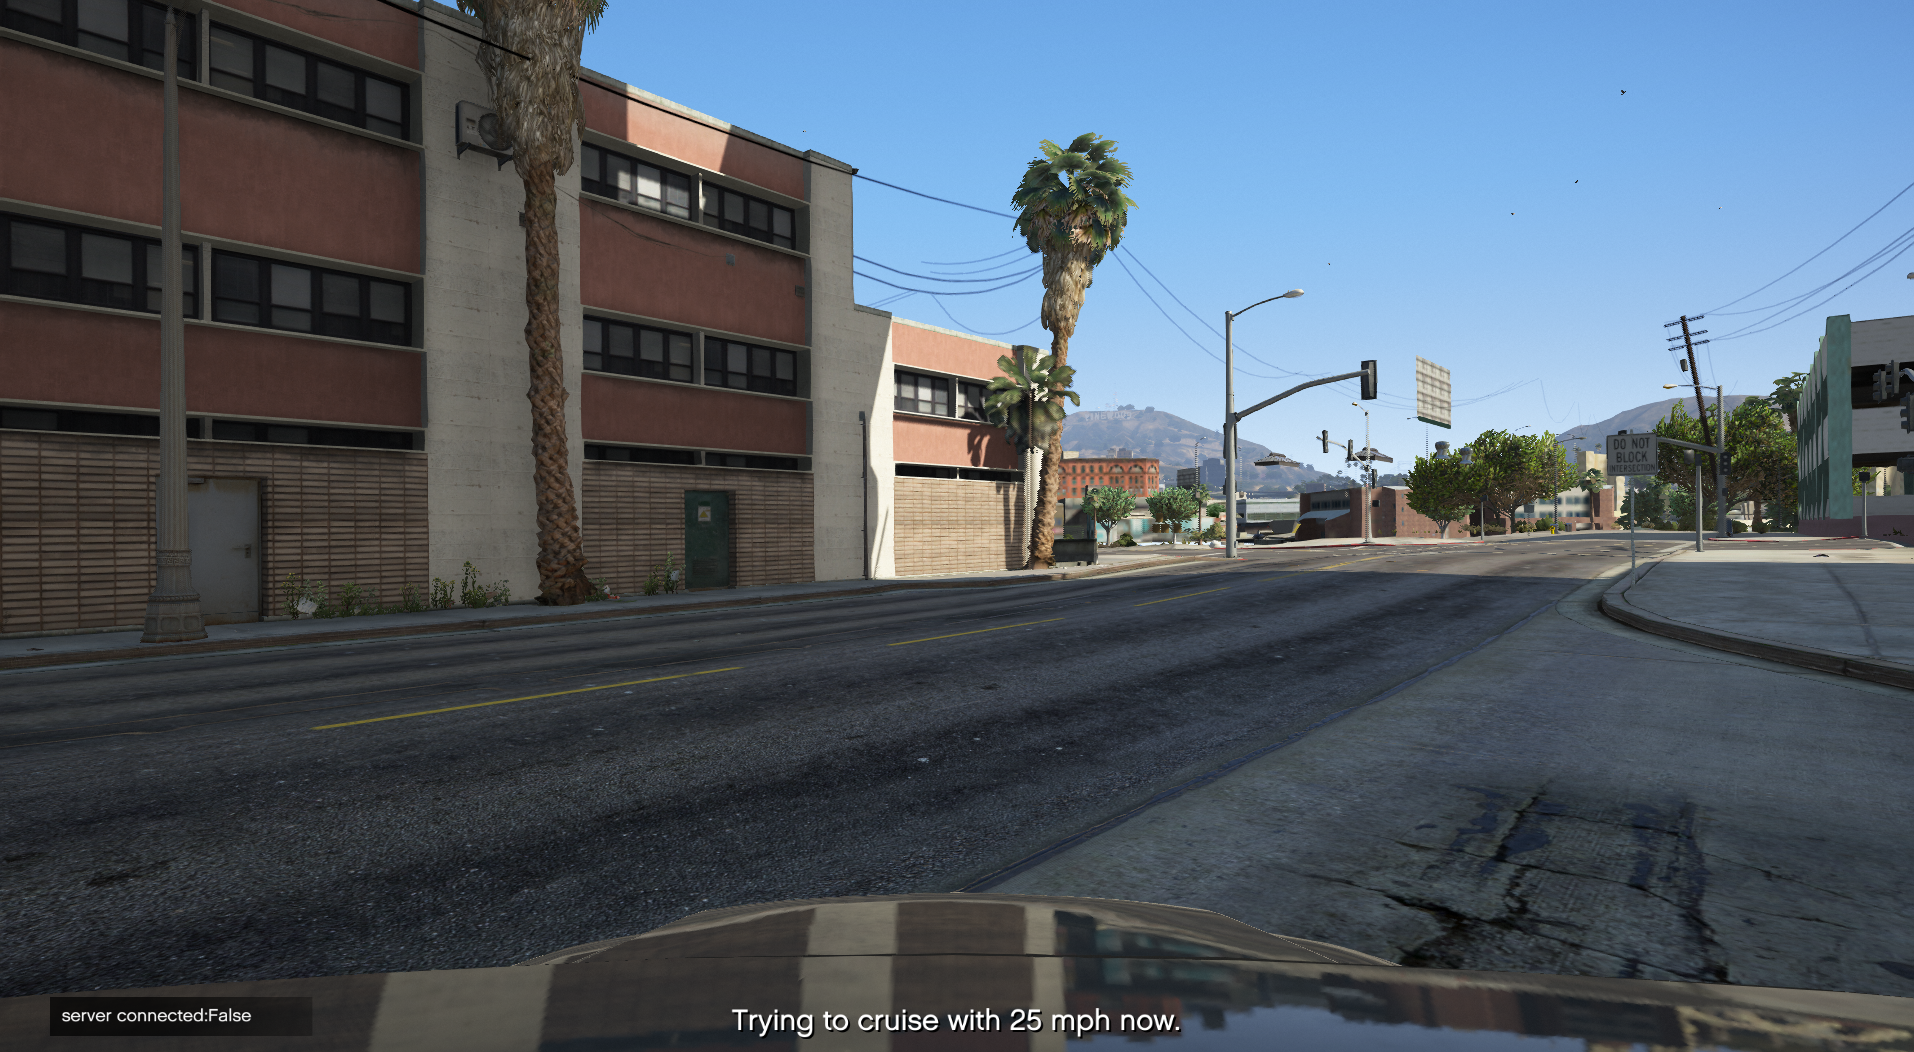
\includegraphics[width=0.48\textwidth,keepaspectratio]{img/gtargbim.png}}\label{gtargbim}}
\hfil
\subfloat[Depth image]{{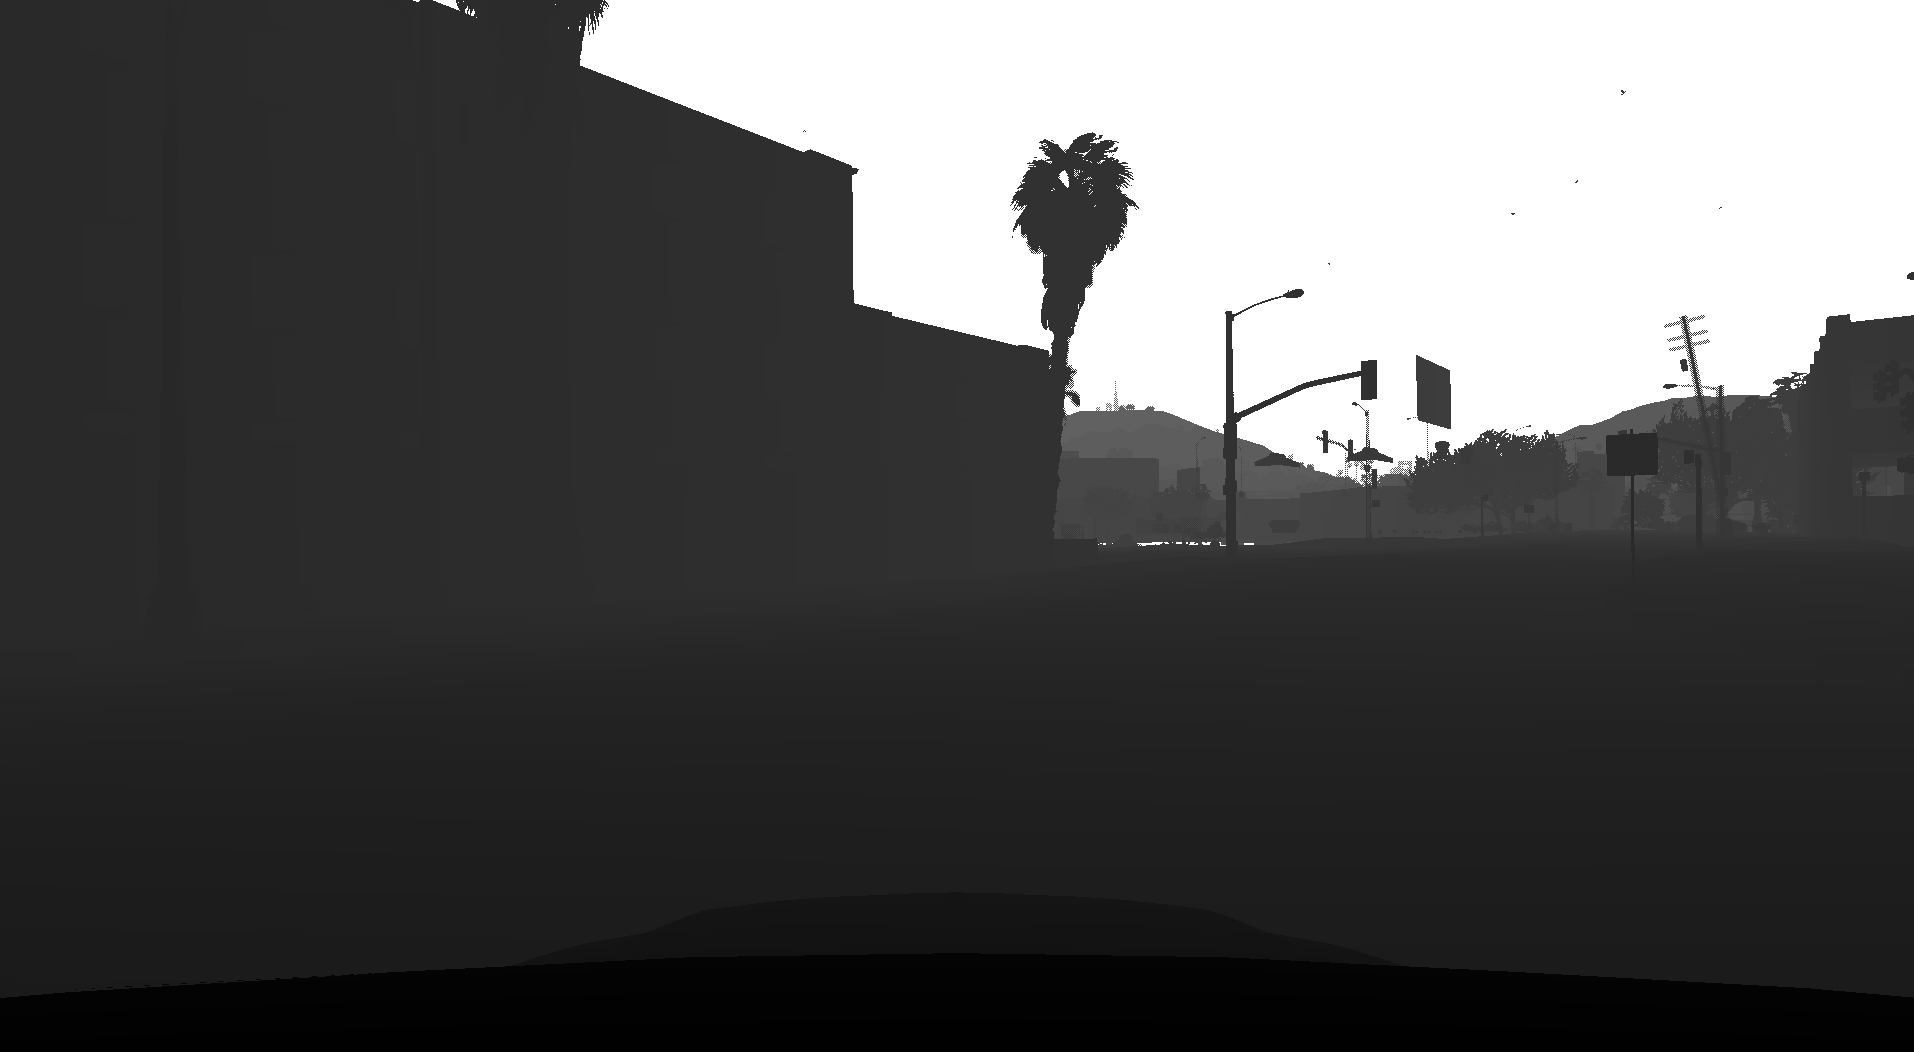
\includegraphics[width=0.48\textwidth,keepaspectratio]{img/gtadepthim.png}}\label{gtadepthim}}
\caption{Example of images from GTA}
\end{figure}

Thanks to Matěj Račinský, who did tremendous work on exploiting Grand Theft Auto and extracting information from it automatically (such as depth, stencil buffer, etc.), we only had to use the data provided by his scripts. The data came in the form of the depth image such as \ref{gtadepthim} from in-game camera and corresponding camera matrix transforming the image to the world coordinates. However, due to the game limitations, it was always possible to capture only one camera at a time and it took non-zero time to switch the cameras to capture another image. Because of these limitations it took about one second of in-game time to capture the full 360\degree{} scene around the car. Data in Valeo dataset produce a full scan at a rate of 10~Hz and since we wanted to match the Valeo data as closely as possible, we simply interpolated positions of the car with 100~ms intervals. This actually created more measurements than depth images, however they are all taken from a different position in the in-game world.

All four virtual cameras sit at the height of one meter from the car center, which later proved to be too low and therefore quite a large portion of the car was reflected in LiDAR-like image. To correct for that, the center of the virtual LiDAR was shifted by 0.75 meters above the camera centers (1.75 meters above the car center).

We don't have intensity information from this LiDAR simulation, so we set intensity to all valid rays as 0.5 (maximal intensity is 1, minimal is 0). The dataset has 14046 LiDAR-like measurements, and it was split into two parts -- training and testing. Training portion of the dataset consists of 8427 measurements, testing contains 5619 measurements. Data from testing portion were not seen by the network during the training phase. The size of the dataset translates into 1404.6 seconds of in-game time that was recorded continuously.

Figure \ref{gtafullpcl} shows an example of the original pointcloud, figure \ref{gtalidarpcl} shows the recreated point cloud from the data from GTA dataset, figure \ref{gtalidardepth} shows an example of a first channel of the data. To ease the viewing, the horizontal stripe of 64$\times$2084 is cut into 4 pieces stacked on top of each other, creating the new size of 256$\times$521.

\begin{figure}
\centering
\subfloat[Full point cloud]{{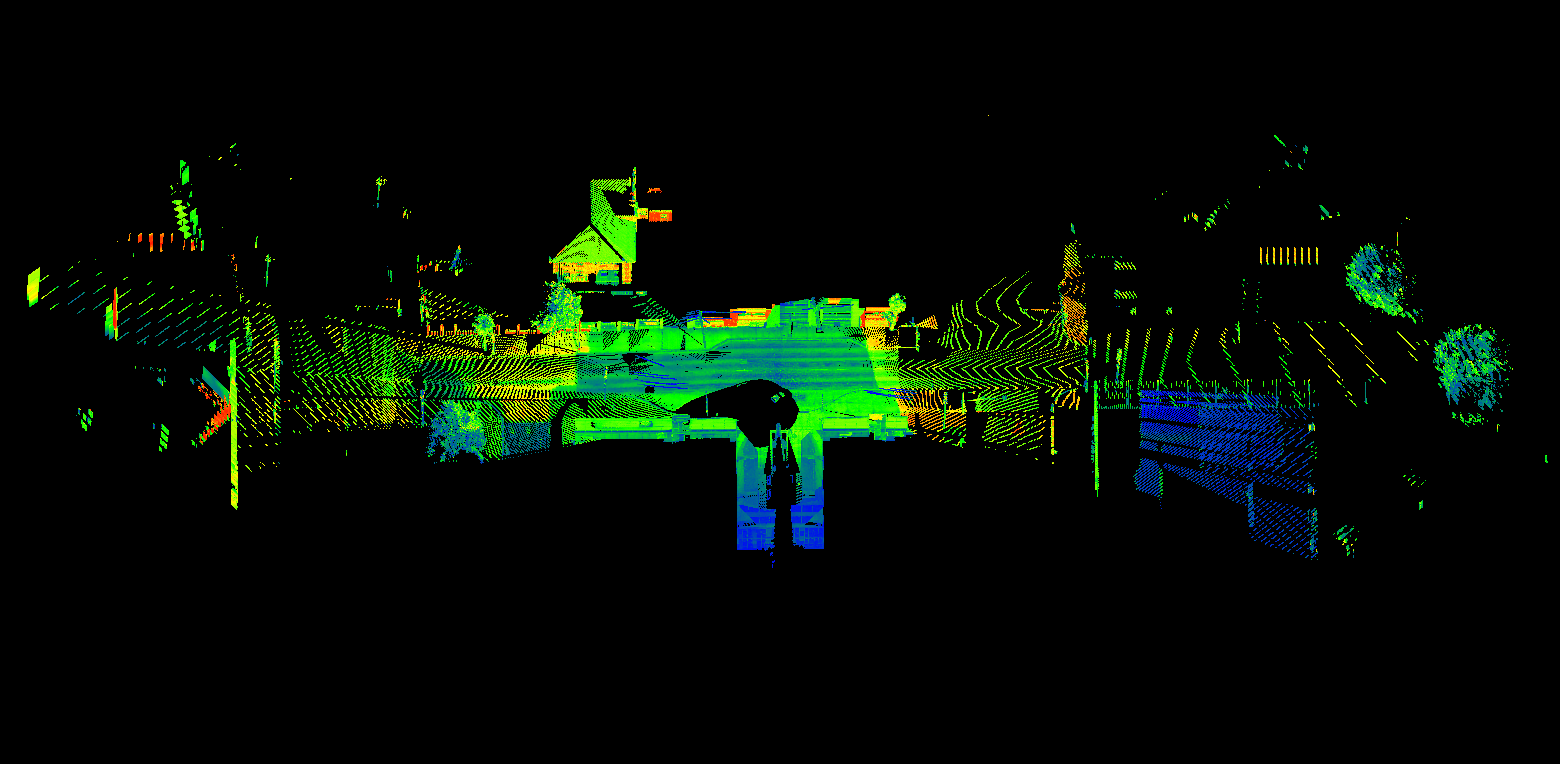
\includegraphics[width=0.48\textwidth,keepaspectratio]{img/gtafullpcl.png}}\label{gtafullpcl}}
\hfil
\subfloat[Reconstructed point cloud]{{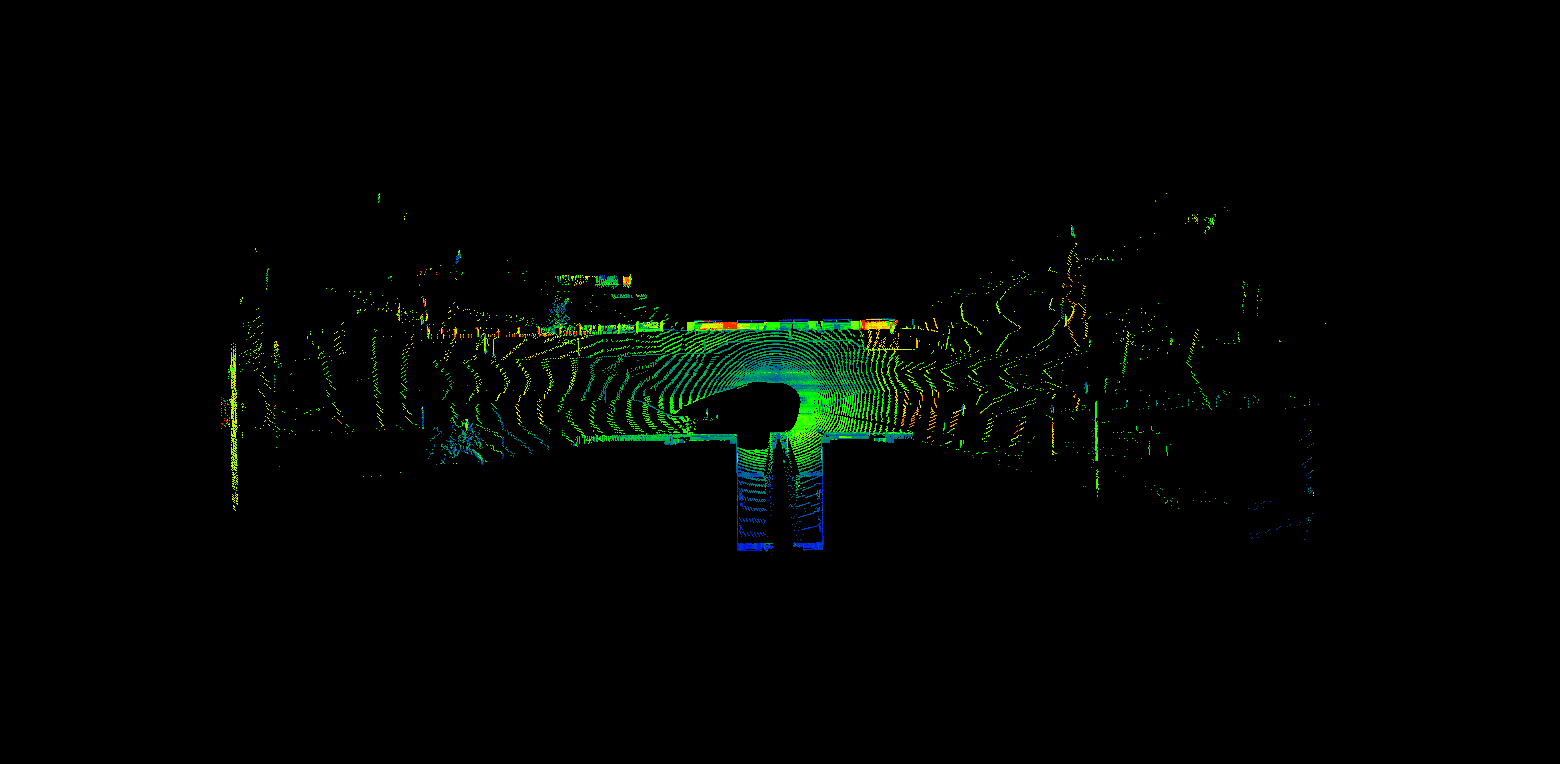
\includegraphics[width=0.48\textwidth,keepaspectratio]{img/gtalidarpcl.png}}\label{gtalidarpcl}}
\caption{GTA point clouds}
\end{figure}

\begin{figure}
\centering
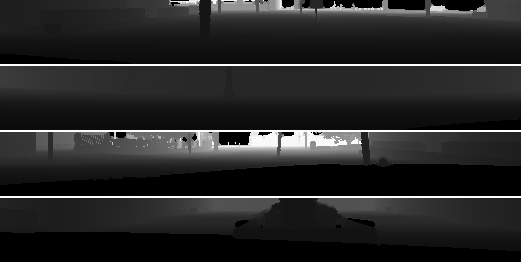
\includegraphics[width=0.98\textwidth,keepaspectratio]{img/gtalidardepth.png}
\caption[First channel of LiDAR-like data from GTA dataset]{First channel of LiDAR-like data from GTA dataset. For easier viewing, the strip of data is divided into 4 equal stripes stacked on top of each other.}
\label{gtalidardepth}
\end{figure}

\subsection{Valeo dataset}
Valeo company provided us with two types of data -- raw and converted. Raw data contained UDP packets from various sensors before any processing with most prominent being Velodyne HDL-64E LiDAR and OXTS xNAV 550 which is a GNSS-aided inertial measurement system. Converted data consisted of point clouds and transformation matrices. Each point cloud corresponded to one full rotation of LiDAR and was already compensated for the movement of the car. The matrices served for transforming particular point clouds into common reference frame. This reference frame was usually the same as the coordinate frame of the first point cloud -- therefore the first point cloud had {\em identity} as this transformation matrix. The origin of the coordinate frame seemed to be in the car center -- we moved the virtual LiDAR center by two meters up to simulate it being on top of the roof of the car.

We decided it would be easier to use {\em converted} data -- mostly because it seemed that it contained precisely the same data as the raw, but without the hassle of parsing and processing Velodyne and OXTS UDP packets. Converted data also contained intensity measurements.

The dataset consists of 22 runs of lengths from 60 to 80 seconds in a cityscape only, resulting in total of 17393 full scans. Training portion of the dataset contains 10435 samples, testing part has 6958 measurements. The data were recorded from 22\textsuperscript{nd} February 2017 till 28\textsuperscript{th} March 2017 with two different cars.

Figure \ref{valeofullpcl} shows an example of the original LiDAR full scan, figure \ref{valeolidarpcl} shows the recreated point cloud from LiDAR-like data and figure \ref{valeolidardepth} shows an example of a first channel of the data. It is partitioned similarly as in figure \ref{gtalidardepth}.


\begin{figure}
\centering
\subfloat[Original LiDAR point cloud]{{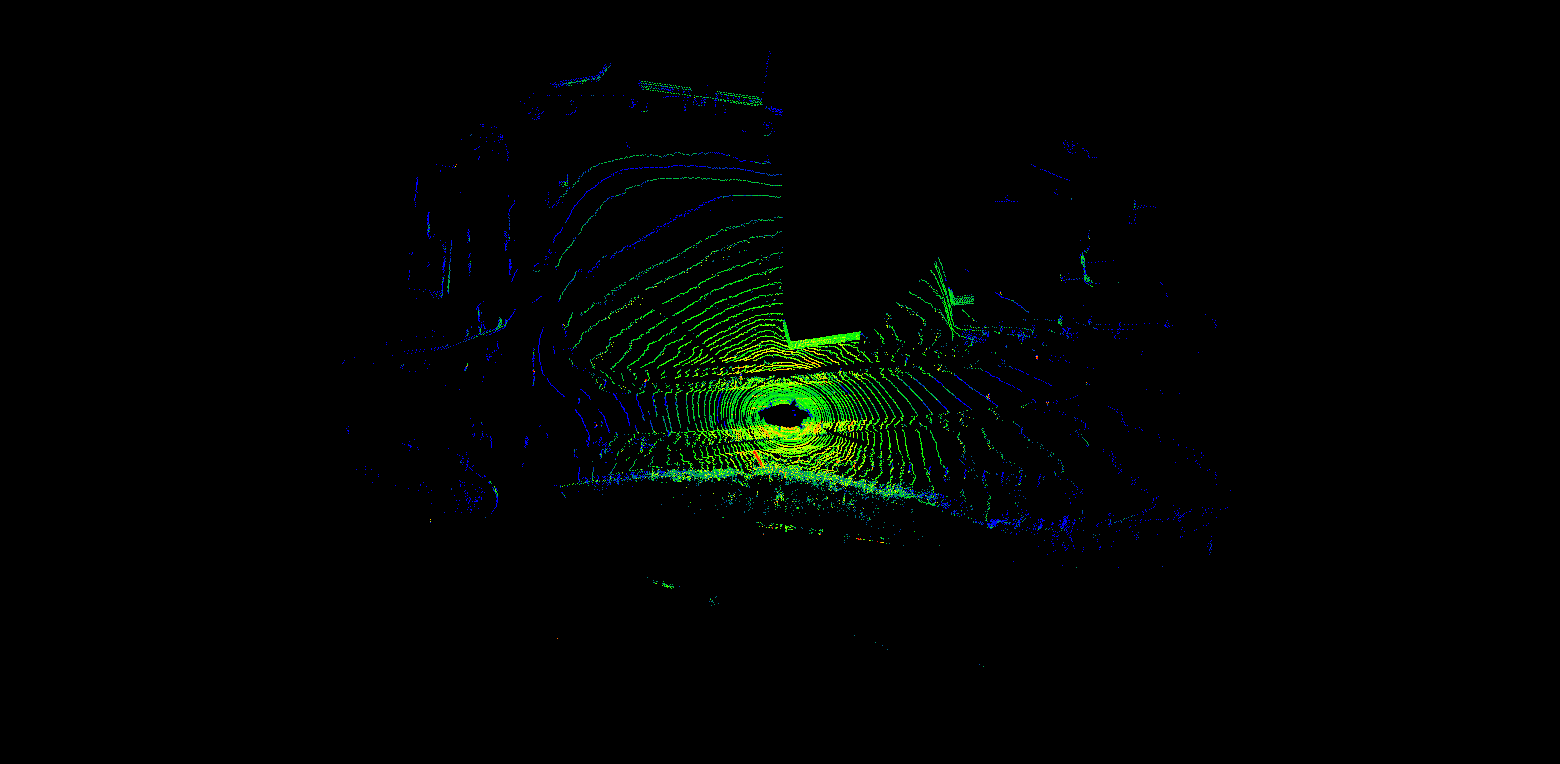
\includegraphics[width=0.48\textwidth,keepaspectratio]{img/valeofullpcl.png}}\label{valeofullpcl}}
\hfil
\subfloat[Reconstructed point cloud]{{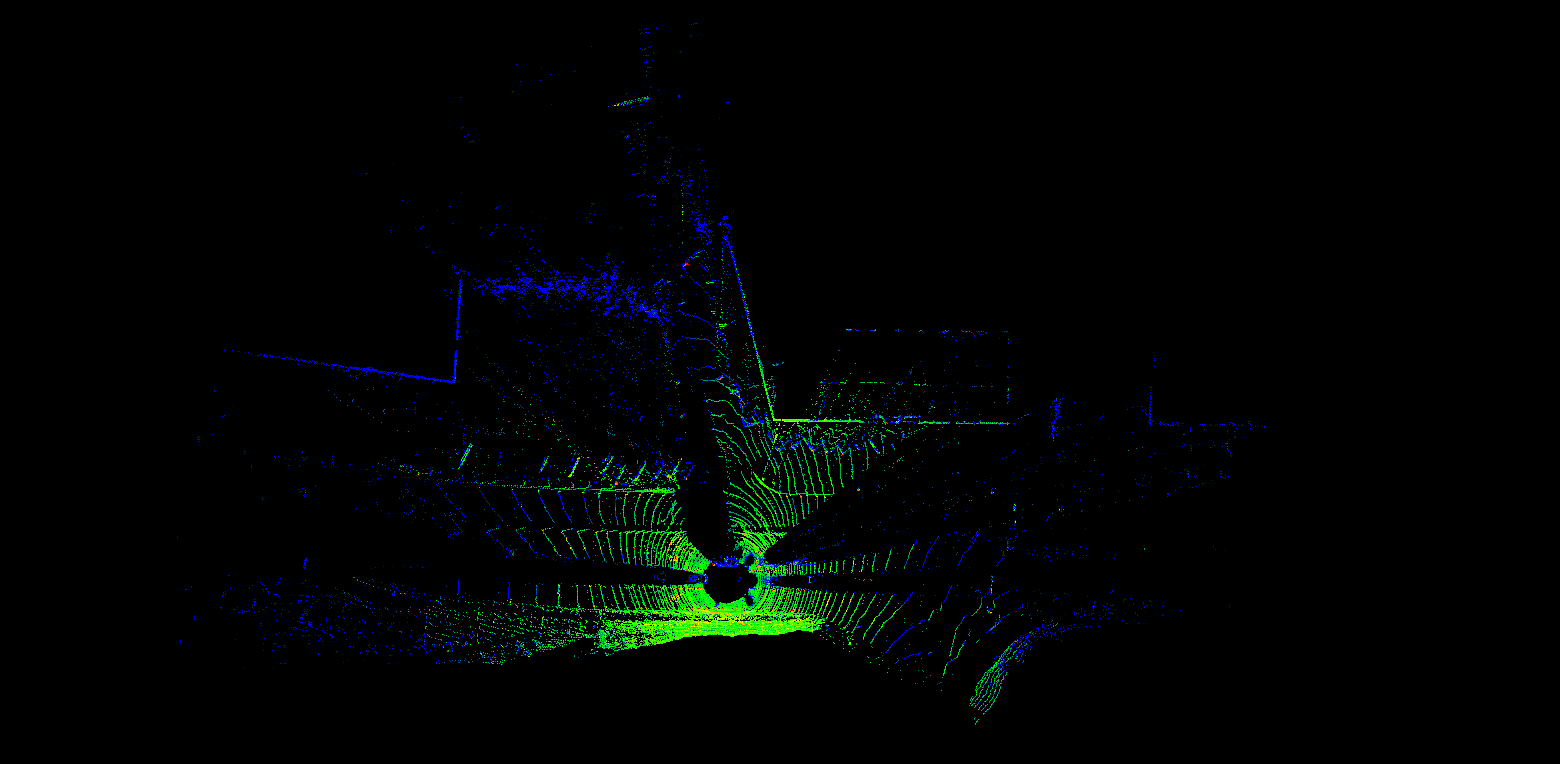
\includegraphics[width=0.48\textwidth,keepaspectratio]{img/valeolidarpcl.png}}\label{valeolidarpcl}}
\caption{Valeo point clouds}
\end{figure}

\begin{figure}
\centering
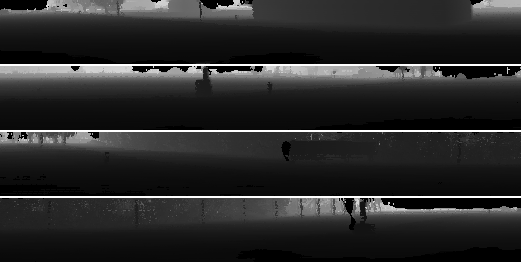
\includegraphics[width=0.98\textwidth,keepaspectratio]{img/valeolidardepth.png}
\caption[First channel of LiDAR-like data from Valeo dataset]{First channel of LiDAR-like data from Valeo dataset. For easier viewing, the strip of data is divided into 4 equal stripes stacked on top of each other.}
\label{valeolidardepth}
\end{figure}


\section{RGB sensors}

\subsection{Grand Theft Auto dataset}

\subsection{KITTI dataset}

\chapter{Programs} \label{programs}

The main program developed for the purpose of this thesis was a Python package \texttt{cycle} implementing modular CycleGAN~\cite{cyclegan} in TensorFlow~\cite{tensorflow} and two programs built on top of this package. This package and associated programs reside in a directory \texttt{mod-cycle-gan} at \url{https://gitlab.fel.cvut.cz/jasekota/master-thesis/tree/master/code/mod-cycle-gan} and will be therefore together referenced as \texttt{mod-cycle-gan}. There is also an utility program written in C++ called \texttt{dat-unpacker} which reads ADTF DAT files used by Valeo company and extracts data from them into an intermediate format similar to the one gathered from GTA. Last portion of code developed for this thesis is a simple Python module (with critical part of the code written in Cython) with simple name \texttt{data-processing}. These three programs/packages will be described more in-depth in following sections.

\section[\texttt{mod-cycle-gan}]{\texttt{mod-cycle-gan} -- Python package \texttt{cycle} and programs \texttt{train.py} and \texttt{test.py}}

Python package \texttt{cycle} is the implementation of CycleGAN~\cite{cyclegan} with large inspiration from GitHub repository of Van Huy at \url{https://github.com/vanhuyz/CycleGAN-TensorFlow}.

\subsection{Exported classes}


\begin{itemize}
\item \texttt{CycleGAN} -- Main class implementing CycleGAN.
\begin{description}
\descitem{\texttt{\_\_init\_\_()}} Constructor of this class takes numerous arguments. First two arguments (\texttt{XtoY, YtoX}) correspond to GANs to be set in cycle fashion (instances of \texttt{nets.GAN} or its subclasses), another two (\texttt{X\_feed, Y\_feed}) are for TFRecords file readers (\texttt{utils.TFReader}) and another two (\texttt{X\_name, Y\_name}) correspond to names of the dataset for pretty printing of logs and Tensorboard messages. Following argument (\texttt{cycle\_lambda}) is a $\lambda$ for cyclic loss function (for more detail see section \ref{cyclegan}). Next argument (\texttt{tb\_verbose}) is a boolean for deciding whether to create summaries for Tensorboard and following argument (\texttt {visualizer}) is a function to use for visualizing the data in Tensorboard -- if this argument is set to \texttt{False} or \texttt{None} then no function will be used for visualisation.

Next four arguments (\texttt{learning\_rate, beta1, steps, decay\_from}) control optimization process -- namely initial learning rate for Adam optimizer~\cite{adam}, parameter beta1 of said optimizer, number of steps (where one step corresponds to one batch) and number of steps after which the learning rate starts to decay to eventually stop at zero. Following argument (\texttt{history}) indicates, whether to use history pool according to~\cite{historypool} and finally, last argument (\texttt{graph}) specifies the computational TensorFlow graph in which the model should be created. If it is left as \texttt{None}, then new graph will be created.
\descitem{\texttt{get\_model()}} This method actually creates the full model in TensorFlow graph. As such, it should be only called once. It sets up all the losses and their respective optimizers. This method has no arguments.
\descitem{\texttt{train()}} This method is the main training loop. The only required argument (\texttt{checkpoints\_dir}) is the top-level checkpoints directory in which a new directory for this session is either created if needed or selected as a loading point in case of retrying training. Next two arguments (\texttt{gen\_train, dis\_train}) specify how often should be generator and discriminator trained within one training step. Next argument (\texttt{pool\_size}) specifies the size of the history pool. Following argument (\texttt{load\_model}) specifies a directory from which to load a saved model if retrying. Note that it is a path relative to top-level checkpoints directory. If this argument is \texttt{None}, new directory with current timestamp is created and new training starts. Next argument (\texttt{log\_verbose}) is a boolean specifying whether to log current loss periodically or not. Next argument (\texttt{param\_string}) specifies string which is a serialized version of arguments with which \hyperref[trainpy]{\texttt{train.py}} script was executed. This string will be saved to checkpoint directory with name \texttt{params.flagfile}. Last argument (\texttt{export\_final}) specifies whether to export final model after training as a binary protobuf used for testing.
\descitem{\texttt{export()}} This method requires two arguments -- first argument (\texttt{sess}) is a session in which a model was run and the second (\texttt{export\_dir}) is a directory in which to save the model. There will be two saved models of names \texttt{\{Xname\}2\{Yname\}.pb} and \texttt{\{Yname\}2\{Xname\}.pb} which can then be used for testing. This method is automatically at the end of the \texttt{train()} method if the last argument (\texttt{export\_final}) was set to \texttt{True}.
\descitem{\texttt{export\_from\_checkpoint()} -- static method} This method is a static counterpart of the \texttt{export()} method. It requires more arguments than method \texttt{export()} because it does not have all the book-keeping information the instance method has. First two arguments (\texttt{XtoY, YtoX}) are instances of GANs with the same model as used for training, another four arguments (\texttt{X\_normer, X\_denormer, Y\_normer, Y\_denormer}) are normalization and denormalization functions to be used for both datasets prior feeding the examples to network and converting them back to useful values. Next argument (\texttt{checkpoint\_dir}) corresponds to checkpoint directory where the model is stored and following argument (\texttt{export\_dir}) specifies directory in which the output models will be saved. Last two arguments (\texttt{X\_name, Y\_name}) correspond to the names of the datasets for easier identification of created models.
\descitem{\texttt{test\_one\_part()} -- static method} This method tests the stored exported model with a NumPy file and saves the important outputs of the network to a new NumPy file. First argument (\texttt{pb\_model}) is a path to an exported binary protobuf model of the network to test. Another argument (\texttt{infile}) specifies the path to the input file to test and next argument (\texttt{outfile}) corresponds to a path of output file. This output file will be a Npz NumPy file with three fields -- \texttt{output} (output generated by corresponding generator), \texttt{d\_input} (value of corresponding discriminator evaluated on input data) and \texttt{d\_output} (value of corresponding discriminator evaluated on output data).

Last argument (\texttt{include\_input}) is a boolean specifying whether to include input data in the output file or not. If set to \texttt{True}, \texttt{outfile} will become larger, however it will be more self-contained.
\end{description}
\item \texttt{utils.TFReader} -- Class for reading TFRecords file, which is a TensorFlow binary format for efficient storage of data and features based on Protobuf.
\begin{description}
\descitem{\texttt{\_\_init\_\_()}} First argument (\texttt{tfrecords\_file}) specifies the path to the TFRecords file to read. Another argument (\texttt{name}) specifies the name of the dataset. This name is rather important, because it needs to be the same as set in TFRecords file \texttt{utils.TFWriter} for parsing of the TFRecords file to be successful. Next argument (\texttt{shape}) is a shape of one example stored in TFRecords file. Since all the data in TFRecords file are stored as flattened arrays, this needs to be set to correct size in order to reshape it to desired size. Next argument (\texttt{shuffle\_buffer\_size}) is passed to the method \texttt{shuffle()} of \texttt{tf.data.Dataset} and as such represents the number of samples used for shuffling. Following two arguments (\texttt{normer, denormer}) are functions operating on tensors for normalizing and denormalizing elements of the dataset (i.e. casting to correct type, squeezing or expanding range, etc.) By default these are identity functions. These functions should be able to accept a keyword \texttt{name} (they are used for exporting). Next argument (\texttt{batch\_size}) is a size of one batch produced by this reader and the last argument (\texttt{num\_threads}) specifies how many threads should be used in operations concerning creating the dataset where applicable.
\descitem{\texttt{feed()}} This method returns new batch of elements from the dataset when run in TensorFlow session. It is used by \texttt{CycleGAN} methods \texttt{get\_model()} and \texttt{train()}. It does not accept any parameters.
\end{description}
\item \texttt{utils.TFWriter} -- Class for creating TFRecords file from NumPy files.
\begin{description}
\descitem{\texttt{\_\_init\_\_()}} The constructor accepts three arguments -- first argument (\texttt{name}) is a name of a dataset. Next argument (\texttt{infiles}) is either a single NumPy file or a list of such files comprising the full dataset. It is expected, that all dimensions except the first one will match within the files. The first dimension represents number of {\em single} elements (with possibly more complex shape, such as $64\times2084\times3$ as is the case in LiDAR-like data used in our experiments) of datasets. Last argument (\texttt{process\_data}) is a function operating on these single elements and tweaking them somehow if needed before storing the data to TFRecords file. The reason, why this argument might be useful (instead of using argument \texttt{normer} of class \texttt{utils.TFReader}) is that this function does not operate on tensors which makes most functions more limiting.
\descitem{\texttt{run()}} This method takes one argument (\texttt{outfile}) specifying path to the output TFRecords file. It will report progress to the default logger (with level \texttt{INFO}) every 10 examples processed.
\end{description}
\item \texttt{utils.DataBuffer} -- Class implementing history pool according to~\cite{historypool}. This class is used by method \texttt{train()} of class \texttt{CycleGAN} and should not be instantiated on its own.
\begin{description}
\descitem{\texttt{\_\_init\_\_()}} Constructor of this class takes three arguments. First argument (\texttt{pool\_size}) manages the size of the pool to be used. It has to be either $-1$ (where essentially there is no pool and this particular instance of the class has no effect) or at least as large as the second argument, \texttt{batch\_size}. Third argument (\texttt{old\_prob}) controls the probability with which the older image is returned by method \texttt{query()} instead of the one that was given. This probability comes to play only when the buffer is filled to its maximum (\texttt{pool\_size}).
\descitem{\texttt{query()}} This method will return the data of the same shape it was fed (by first argument -- \texttt{data}). If the internal buffer was already filled, then it will replace randomly elements of the data forming a batch with a probability given in the constructor by argument \texttt{old\_prob} and swaps the elements it replaced into its buffer in the places of the elements that are used in replacement. If the buffer is not filled yet, it will only store the elements from \texttt{data} argument and not replace them.

Second argument (\texttt{cur\_step}) indicates the global step of the training process in order to be able to return the same data for the same step (for example, if training uses multiple training step for discriminator or generator).
\end{description}
\item \texttt{nets.BaseNet} -- Base class for mapping networks (Generator and Discriminator). This class encapsulates mapping network and if you want to create your own mapping network and feel limited by the capabilities of this, you should subclass it and re-implement method \texttt{transform()}.
\begin{description}
\descitem{\texttt{\_\_init\_\_()}} Constructor of this class takes five arguments. First argument (\texttt{name}) is a name of the network as it will appear in TensorFlow computational graph and this name will encapsulate all of the operations of the network. Second argument (\texttt{network\_desc}) is a string describing layers of the network and will be dissected in more detail at subsection \ref{networkdesc}. Third argument (\texttt{is\_training}) is a boolean indicating whether the network is in a training or testing mode. This is mostly important for norms.

Next argument (\texttt{weight\_lambda}) is a $\lambda$ of weight term of the loss function for this particular network. This was motivated by having lot of networks with skip connection where we wanted to make only small changes to the image and thus minimizing the weights of generators and therefore generating only small perturbations.

Last argument (\texttt{norm}) is a type of normalization used in network layers. Can be either \texttt{'instance'}~\cite{instancenorm}, \texttt{'batch'}~\cite{batchnorm} or anything else for no normalization between layers. It does not make any sense to use different normalizations within one network so this setting can be made global for the whole network.
\descitem{\texttt{\_\_call\_\_()}} This is the way how the mapping induced by this object will be called. It essentially just wraps the call to \texttt{transform()} method inside a variable scope of the name specified by the first argument of the constructor (\texttt{name}) and collects all the trainable variables into the list called \texttt{variables}. This book-keeping is done to ease the subclassing since now the only method to be replaced is \texttt{transform()} without the need to worry about collecting all the trainable variables and placing it under same particular variable scope.
\descitem{\texttt{transform()}} This method accepts one argument (\texttt{data}) -- tensor that will be transformed by the network. It is the core of the class \texttt{nets.BaseNet} and if you decide to write your own mapping network by subclassing, this method {\em must} be implemented. By default, it creates the mapping network according to the argument \texttt{network\_desc} supplied to the constructor. The syntax of this simple string will be more in depth explained at subsection \ref{networkdesc}.
\descitem{\texttt{weight\_loss()}} This method return weight loss of the mapping network defined by equation \ref{wloss}, where $\theta_F$ is a set of trainable variables of a mapping function $F$ represented by this object, $\lambda_{\text{w}F}$ is a multiplier denoting the contribution of this loss term to the overall loss function and $L_{\text{w}F}$ is a loss term returned by this method.

\begin{equation}
L_{\text{w}F} = \lambda_{\text{w}F} \frac{1}{|\theta_F|} \sum_{\bm{w} \in \theta_F} \norm{\bm{w}}_2^2
\label{wloss}
\end{equation}

\end{description}

\item \texttt{nets.GAN} -- Implementation of Generative Adversarial Network (GAN)~\cite{origgan}. Uses original loss functions.

\begin{description}
\descitem{\texttt{\_\_init\_\_()}} First two arguments (\texttt{gen, dis}) of the constructor are the mapping networks -- generator and discriminator (in the original paper $G(\cdot)$ and $D(\cdot)$), where discriminator should produce real number in a range [0; 1] due to the way how is loss function defined. If the discriminator function's output is of higher dimension than one, then the appropriate loss function is computed in each dimension independently and the final loss is arithmetical mean of these loss functions. If discriminator network is a convolutional network, one can think of this as the loss computed at different patches extracted by the network.

Next two arguments (\texttt{in\_shape, out\_shape}) specify input and output shapes of generator {\em without} the batch size. Though this information could be easily obtained from the generator function, it is there mostly to check that the shapes are correct and indeed what you intended them to be. Next two arguments (\texttt{gen\_lambda, dis\_lambda}) are $\lambda$s that correspond to the weight of the respective terms in the final loss function.
\descitem{\texttt{gen\_loss()}} This method expects one argument -- data of \texttt{in\_shape} that will be fed to generator to produce the loss term of the generator according to the equation \ref{gangenloss}, where $\lambda_G$ is a multiplier denoting the contribution of this loss term, $G(\cdot)$ is a generator mapping, $D(\cdot)$ is a discriminator mapping, $\bm{x}$ is input data for generator mapping and $L_{G}$ is a loss term returned by this method.

\begin{equation}
L_{G} = -\lambda_G\log(D(G(\bm{x})))
\label{gangenloss}
\end{equation}

Note, that the original formulation of the generator loss function by \cite{origgan} is slightly different (as seen in the equation \ref{origgangenloss} where all the symbols have the same meaning as in the equation \ref{gangenloss}), however it was suggested in the same paper, that the formulation \ref{gangenloss} is equivalent with an important advantage of stronger gradients early in the training process.

\begin{equation}
L_{G} = \lambda_G\log(1 - D(G(\bm{x})))
\label{origgangenloss}
\end{equation}

\descitem{\texttt{dis\_loss()}} This method takes two arguments (\texttt{real, fake}) which are both of the \texttt{out\_shape} -- \texttt{real} is a real sample from the target distribution and \texttt{fake} is a result of applying $G(\cdot)$ to a sample from the input distribution. This method then computes the discriminator term of the loss function specified by the equation \ref{gandisloss}, where $\lambda_D$ is a multiplier denoting the contribution of this loss term, $D(\cdot)$ is a discriminator mapping, $\bm{\hat{x}}$ corresponds to \texttt{real} argument, $\bm{y}$ corresponds to \texttt{fake} argument and $L_D$ is a loss term returned by this method. Original paper was maximizing the same function without minus sign, and since we are minimizing all terms of the loss functions, we added minus in front of the loss function. The division by 2 is there only to scale both terms equally.

\begin{equation}
L_D = -\frac{\lambda_D}{2} (\log(D(\bm{\hat{x}})) + \log(1 - D(\bm{y})))
\label{gandisloss}
\end{equation}

\end{description}

\item \texttt{nets.LSGAN} -- Implementation of Least Squares GAN~\cite{lsgan}. This is a subclass of \texttt{nets.GAN} and as such all of the methods accept the same arguments. The only difference is in the equations governing the computation of respective terms of the loss function in methods \texttt{gen\_loss()} and \texttt{dis\_loss()}.
\begin{description}
\descitem{\texttt{gen\_loss()}} This method implements the generator loss function according to the equation \ref{lsgangenloss}. The meaning of the used symbols is the same as in equation \ref{gangenloss}. The reason for number 0.9 comes from the label smoothing proposed by~\cite{improvedgan,smooth}.
\begin{equation}
L_G = \lambda_G \norm{D(G(\bm{x})) - 0.9}_2^2
\label{lsgangenloss}
\end{equation}
\descitem{\texttt{dis\_loss()}} This  method implements the discriminator loss function according to the equation \ref{lsgandisloss}. The meaning of the used symbols is the same as in equation \ref{gandisloss}.
\begin{equation}
L_D = \frac{\lambda_D}{2} (\norm{D(\bm{\hat{x}}) - 0.9}_2^2 + \norm{D(\bm{y})}^2)
\label{lsgandisloss}
\end{equation}

\end{description}
\item \texttt{nets.WGAN} -- Implementation of Wasserstein GAN with gradient penalty \cite{wgan}. This is a subclass of \texttt{nets.GAN} as well, however it introduces one more term to the loss function, so called gradient penalty. This is implemented in method \texttt{grad\_loss()}.
\begin{description}
\descitem{\texttt{\_\_init\_\_()}} The constructor takes the same arguments as the constructor of \texttt{nets.GAN} with one more argument (\texttt{grad\_lambda}) specifying the weight of the gradient penalty.
\descitem{\texttt{gen\_loss()}} This method implements the generator loss function according to the equation \ref{wgangenloss}. The meaning of the symbols is the same as in equation \ref{gangenloss}.
\begin{equation}
L_G = -\lambda_GD(G(\bm{x}))
\label{wgangenloss}
\end{equation}
\descitem{\texttt{dis\_loss()}} This method implements the discriminator loss function according to the equation \ref{wgandisloss}. The meaning of the used symbols is the same as in equation \ref{gandisloss}. Note that the gradient penalty term of the loss function is computed in the method \texttt{grad\_loss()}
\begin{equation}
L_D = \frac{\lambda_D}{2}(D(\bm{y}) - D(\bm{\hat{x}}))
\label{wgandisloss}
\end{equation}

\descitem{\texttt{grad\_loss()}} This method computes the gradient penalty term according to the equation \ref{wgangradloss}, where $\lambda_{DGP}$ is a multiplier denoting the contribution of the gradient penalty term to the overall loss, $\bm{\tilde{x}} = \epsilon\bm{\hat{x}} + (1-\epsilon)\bm{y}$, $\epsilon$ is a random number from [0,1] and $L_{DGP}$ is a loss term returned by this method.

\begin{equation}
L_{DGP} = \lambda_{DGP}(\norm{\nabla_{\bm{\tilde{x}}}D(\bm{\tilde{x}})}_2 - 1)^2
\label{wgangradloss}
\end{equation}

\descitem{\texttt{full\_dis\_loss()}} This method computes the full loss of the discriminator, $L_{DGP} + L_D$.
\end{description}
\end{itemize}

\subsubsection{Parameterization of the mapping networks by \texttt{network\_desc}} \label{networkdesc}
The mapping network could be easily parameterized by a special \texttt{network\_desc} string. This string comprises of layers separated by semicolon (\texttt{';'}). All layers comprise of letter from \{\texttt{'c', 'b', 'r'}\} specifying the layer type, followed by hyphen (\texttt{'-'}) and list of integer parameters specific to particular layer each of them separated by hyphen as well. The last part of a layer is again a letter from \{\texttt{'r', 't', 'l', 's', 'i'}\} specifying the used activation function for this particular layer. All of the trainable variables are initialized using Xavier initializer~\cite{xavier} in order to keep the scale of the gradients approximately the same across all layers. Normalization (either instance or batch) is always used before applying activation function. Note that the parameterization using this notation is rather simple and does not allow all possible configurations of specified layers. If you desire finer control over created layers, then using this \texttt{network\_desc} string is not ideal for you.

The tail of the \texttt{network\_desc} string after last semicolon specifies output operation and could be any number of the letters from the set \{\texttt{'s', 'c', 'a'}\}. These output operations are chained in the order in which they appear in the tail of the \texttt{network\_desc} string.

\paragraph{Layers description}
\begin{description}
\descitem{\texttt{'c'} -- 2D Convolutional layer~\cite{convnet}} This layer accepts {\em three} integer arguments -- first argument is a kernel size (the kernel will have square shape), second argument is a stride (same in all directions) used in the convolution and third argument specifies the number of filters used (number of channels in the output). For example the string \texttt{'c-7-1-64-r'} specifies the convolutional layer with kernel of size 7, stride 1, 64 output channels and ReLU~\cite{relu} used as activation function.
\descitem{\texttt{'b'} -- 2D Convolutional ResNet~\cite{resnet} block} This layer creates a ResNet block and accepts {\em two} integer arguments. First argument is a kernel size of each layer comprising this block and second argument specifies the number of repetitions of this convolutional layer. Since ResNet block requires the input and output simension to match, stride is implicitly set to 1 and number of the output channels is the same as the number of the input channels. For example, the string \texttt{'b-3-2-r'} specifies the most classical ResNet block comprising of two convolutional layers with kernel size 3, stride 1 and ReLU activation in between of those two layers.
\descitem{\texttt{'r'} -- Resize and 2D Convolutional layer~\cite{resizeconv}} This layer was originally deconvolutional~\cite{deconv} layer, however to mitigate checkerboard artifacts stemming from using deconvolutional layer~\cite{resizeconv}, we decided to use instead resize and convolutional layer. It accepts {\em three} integer arguments and one float argument. First three arguments correspond to the same arguments as regular convolutional layer and last argument corresponds to coefficient of resizing. The resizing is done using method \texttt{tf.image.resize\_images} with resize method \texttt{tf.image.ResizeMethod.NEAREST\_NEIGHBOR}. The number of channels after resizing stays the same as number of channels in the input image. For example, the string \texttt{'r-3-1-32-2-r'} will first resize the input image making it twice as large as input and then perform convolutional operation with kernel of size 3, stride 1, 32 output channels and ReLU as activation function.
\end{description}

\paragraph{Available activation functions}
\begin{itemize}
\item \texttt{'r'} -- Rectified Linear Unit (ReLU)~\cite{relu}
\item \texttt{'l'} -- Leaky Rectified Linear Unit (Leaky ReLU)~\cite{leakyrelu}
\item \texttt{'t'} -- Hyperbolic tangent function defined by $\tanh(x) = \frac{e^x - e^{-x}}{e^x + e^{-x}}$
\item \texttt{'s'} -- Sigmoid function defined by $S(x) = \frac{e^x}{e^x + 1}$
\item \texttt{'i'} -- Identity, no nonlinear activation function is used.
\end{itemize}

\paragraph{Output operation}
These operations are chained in order in which they appear in the tail of the \texttt{network\_desc}. Note, that this part of the \texttt{network\_desc} can be empty if you don't want to use any special output operation.
\begin{itemize}
\item \texttt{'s'} -- Sums the current output with input to the whole mapping network.
\item \texttt{'c'} -- Clip the output of the whole network to the range [-1; 1].
\item \texttt{'a'} -- Use activation function on the output. Since the operating range for most of the networks is [-1; 1], the only activation function that {\em makes sense} to use is $\tanh$, so this function will be used.
\end{itemize}

\paragraph{Example of the full network}
The full network could be for example parameterized by string \texttt{'c-7-1-64-r;c-5-2-128-r;b-3-3-r;r-5-1-64-2-r;c-7-1-3-t;sc'}. This network consists of two regular convolutional layers with kernel sizes 7 and 5, strides 1 and 2 and having 64 and 128 output channels. Both of these layers use ReLU as activation function. Convolutional layers are then followed by one ResNet block with three convolutional layers and kernel size 3 and again, ReLU is used. Next resize operation follows which creates the image double the size and is followed by another two convolutional layers with kernel sizes 5 and 7, both strides equal to 1 and having 64 and 3 output channels. First of these convolutional layers is followed by ReLU activation function, the second one uses $\tanh$ as activation. Output of the last convolutional layer is then added to the original input and this sum is then clipped to the range [-1; 1]. The described mapping network (with input size (1, 64, 2084, 3) since this is one of the generators we tested) is shown at the figure \ref{netdescfig}.

\begin{figure}
\caption[Example of the network created by \texttt{network\_desc} string]{Example of the network created by \texttt{network\_desc} string \texttt{'c-7-1-64-r;c-5-2-128-r;b-3-3-r;r-5-1-64-2-r;c-7-1-3-t;sc'}}
\label{netdescfig}
\end{figure}

\section[\texttt{dat-unpacker}]{\texttt{dat-unpacker} -- C++ utility}

\section[\texttt{data-processing}]{\texttt{data-processing} -- Python package}

\chapter{Experiments} \label{experiments}

\section{CycleGANs with depth data}

We proposed a set of experiments in order to determine which of the GAN variants performed better for the LiDAR-like images in the CycleGAN~\cite{cyclegan} setting. Therefore all of the experiments were the same except the used loss functions for generator and discriminators. There were altogether six experiments -- original GAN~\cite{origgan}, LSGAN~\cite{lsgan} and WGAN-GP~\cite{wgan-gp} with and without self-regularization~\cite{historypool} term in the generators' loss function. We used mini-batches of size 4 (due to the memory limit of used GPUs) and trained all the networks for 80000 steps resulting in approximately 37 runs through all the training data for GTA dataset and about 32 runs for Valeo dataset. It makes no sense to use the term epoch in the setting of two different dataset with various magnitudes.

The only difference in the architecture was the use of Layer normalizations~\cite{layernorm} for the WGAN-GP instead of Batch normalizations~\cite{batchnorm} for the GAN and LSGAN. This was motivated by the explicit mention of hurting the training process with batch normalization for WGAN-GP~\cite{wgan-gp}.

The CycleGAN was trained using {\em three} training steps for the discriminators for every training step of the generators. This was to ensure the proper training of the discriminator in order to be able to provide good gradients for the training phase of the generators. The Adam optimizer with initial learning rate of 0.0002 and $\beta_1$ parameter of 0.5 was used and after half of the training steps (40000), the learning rate was linearly decreasing until zero at the end of the training.

The structure of the generator networks can be seen at the figure \ref{genstruct}. Note, that the ResNet~\cite{resnet} block is repeating 6 times. Dark blue node indicates input LiDAR-like image, light blue node indicates output LiDAR-like image and each arrow represents flow of the data of specified shape. Green nodes represent convolutional layers and yellow layers represent resize and convolution blocks, which consist of first resizing the data twice (not affecting the number of channels and samples in the mini-batch) and then performing convolution. The structure of the generators was largely inspired by the structure of the generators used by the original paper~\cite{cyclegan}.

\begin{figure}
\centering
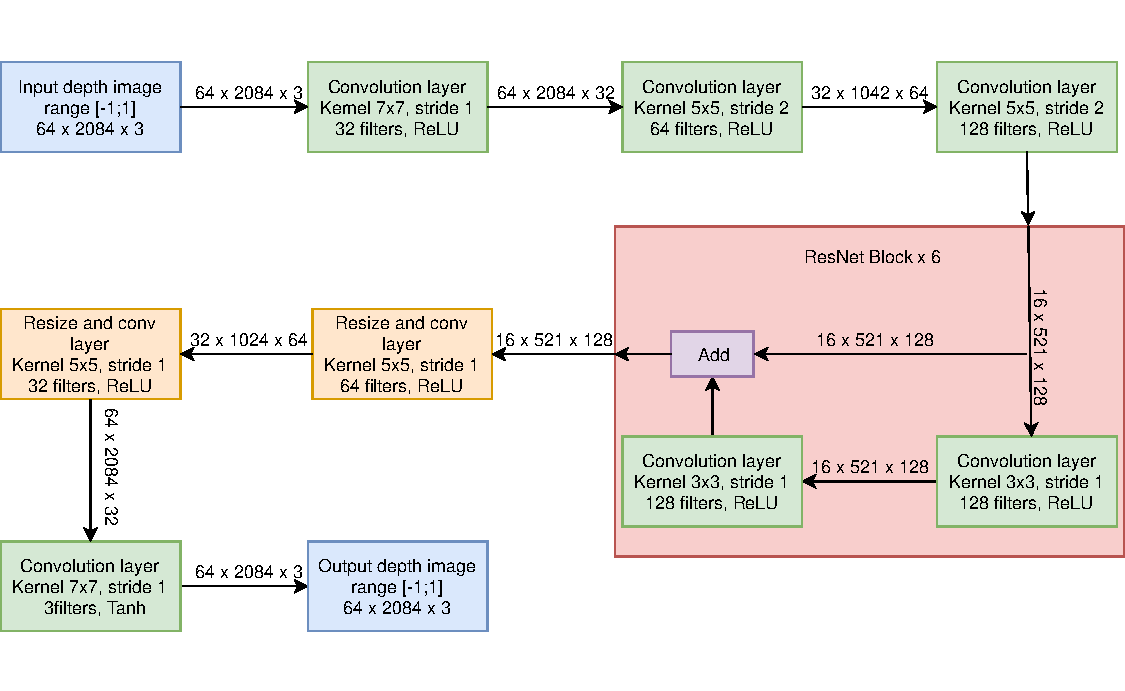
\includegraphics[keepaspectratio, width=0.98\textwidth]{img/gen.pdf}
\caption{Structure of the used generators}
\label{genstruct}
\end{figure}

The structure of the used discriminator can be seen at the figure \ref{disstruct}. Coloring is the same as in the figure \ref{genstruct}, the gray node corresponds to the fully-connected layer.

\begin{figure}
\centering
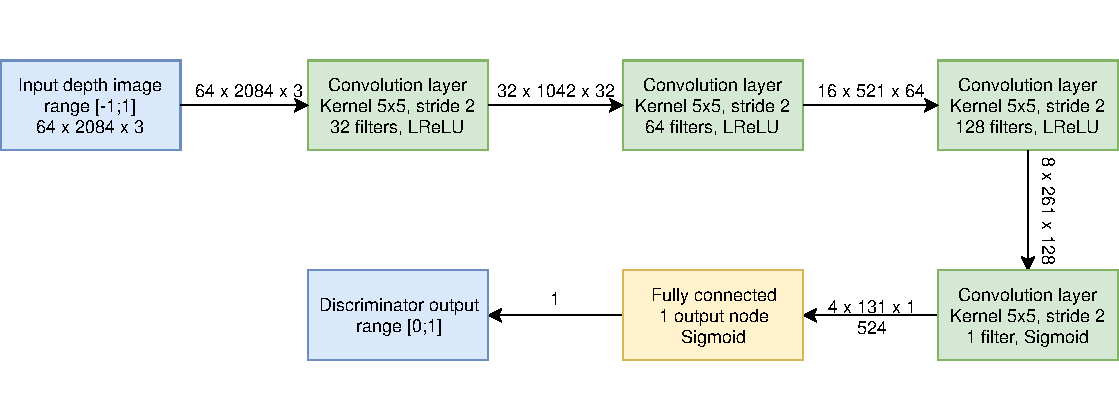
\includegraphics[keepaspectratio, width=0.98\textwidth]{img/disc.pdf}
\caption{Structure of the used discriminators}
\label{disstruct}
\end{figure}

The feature map for the self-regularization term of the generators' loss functions was formulated as follows -- if the pixel corresponding to the particular ray was valid (third channel) in both depth images (original and converted by the generator), then the feature corresponding to that pixel was its depth and intensity (i.e. identity on the first two channels), but if it was not valid in either of the depth images, then the feature map would return tuple (0, 0). The feature map had the shape of $64\times2084\times3$ as an input and $64\times2084\times2$ as its output shape.

All of the experiments used the history pool~\cite{historypool} with the size of the pool being 50. All of the trainable variables in the networks were initialized using the Xavier~\cite{xavier} initialization. The other important hyperparameters are: $\lambda_D = 1$, $\lambda_G = 1$, $\lambda_{cyc} = 3$, $\lambda_{GP} = 3$ (where applicable), $\lambda_{reg} = 3$ (where applicable).

\subsection{Results}

This subsection will show the examples of the results generated by the trained generators from the CycleGAN model. Figure \ref{evalcmpg2v} shows data generated from the testing portion of the GTA dataset transformed into Valeo dataset by the means of different GANs used within CycleGAN model. Figure \ref{evalcmpg2vcutout} shows the same data, but only small part of the images is shown to ease the viewing. Note that while the part displayed in the depth and intensity images show the {\em same} part of the data, the portion displayed in the point cloud section does not correspond to the same part of the scene. The figures \ref{evalcmpv2g} and \ref{evalcmpv2gcutout} have the same layout as figures \ref{evalcmpg2v} and \ref{evalcmpg2vcutout}, only they show the data transformed from the testing portion of the Valeo dataset to GTA dataset.

For more data see the contents of enclosed DVD, as described in the appendix \ref{cd}.

\begin{figure}
\begin{tabular}{L|III}
 & \textbf{Depth} & \textbf{Intensity} & \textbf{Point cloud} \\
Original & 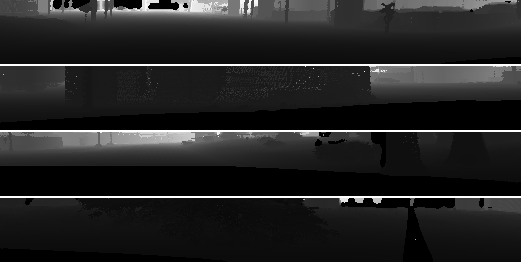
\includegraphics[keepaspectratio, width=\linewidth]{img/gta2valeo_depthorig.png} & 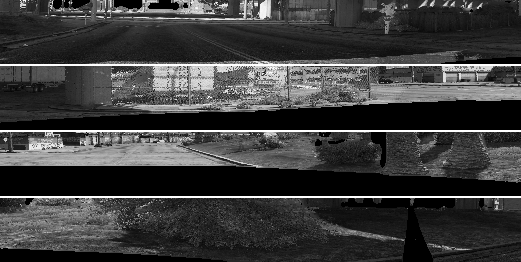
\includegraphics[keepaspectratio, width=\linewidth]{img/gta2valeo_intenorig.png} & 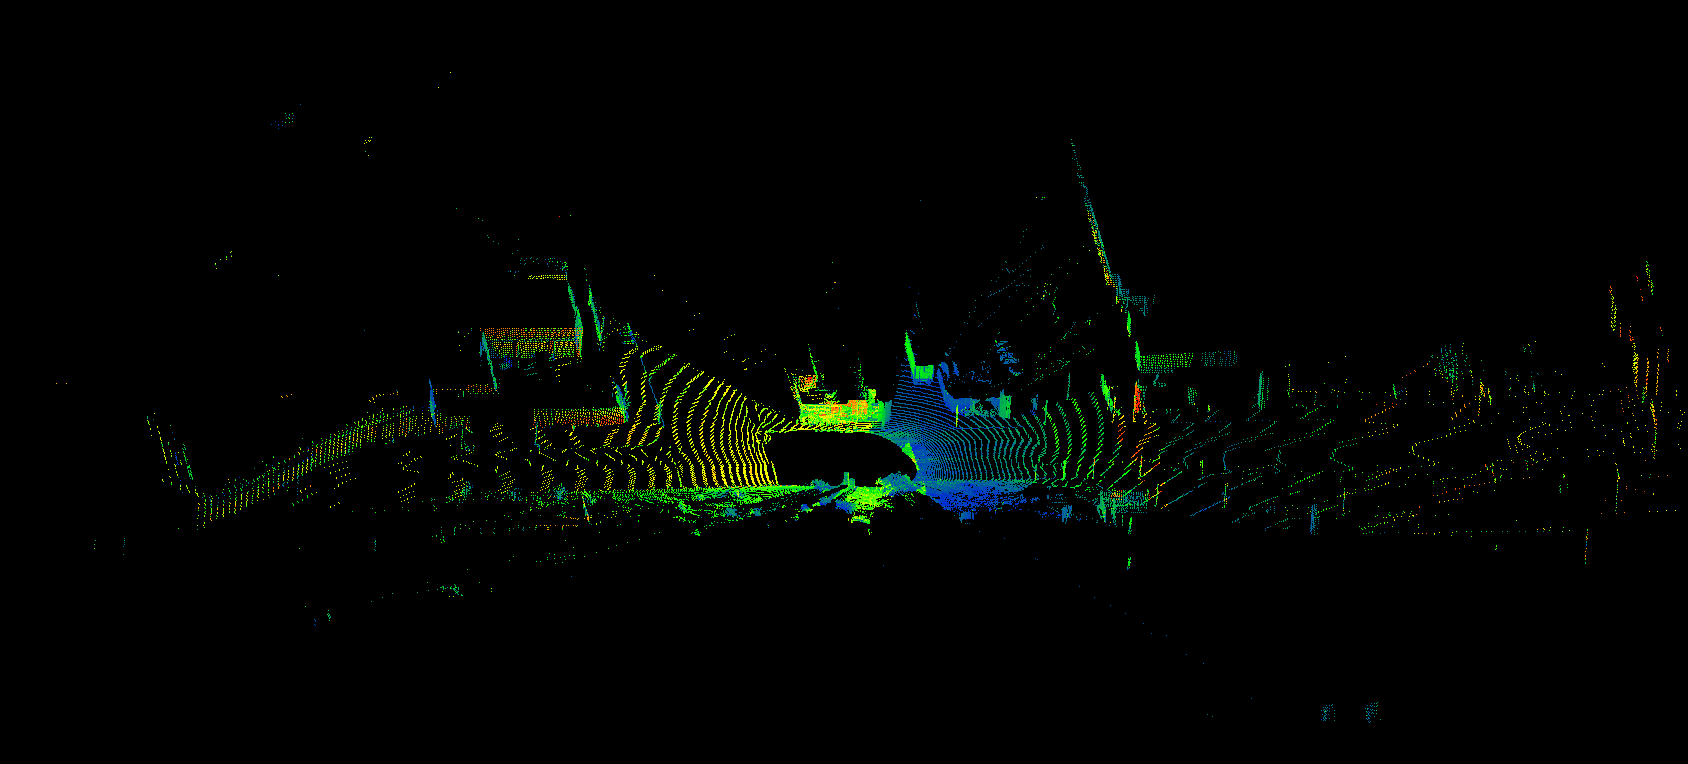
\includegraphics[keepaspectratio, width=\linewidth]{img/gta2valeo_pclorig.png} \\
GAN\linebreak{}No Self-reg & 
\includegraphics[keepaspectratio, width=\linewidth]{img/gta2valeo_depthgannosr.png} & 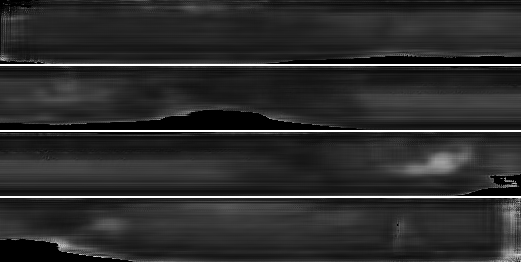
\includegraphics[keepaspectratio, width=\linewidth]{img/gta2valeo_intengannosr.png} & 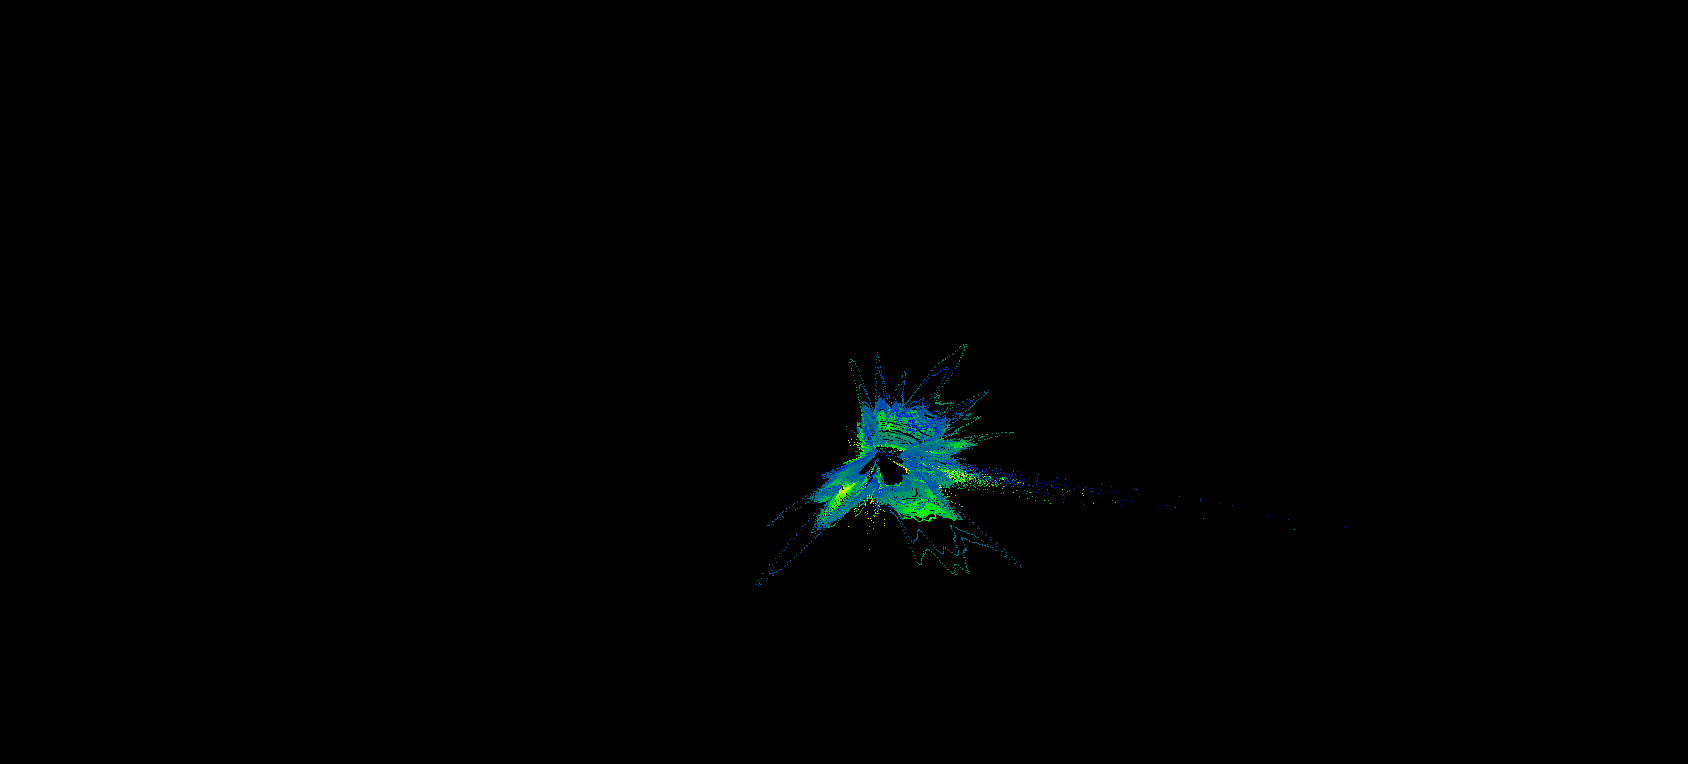
\includegraphics[keepaspectratio, width=\linewidth]{img/gta2valeo_pclgannosr.png} \\
GAN\linebreak{}Self-reg & 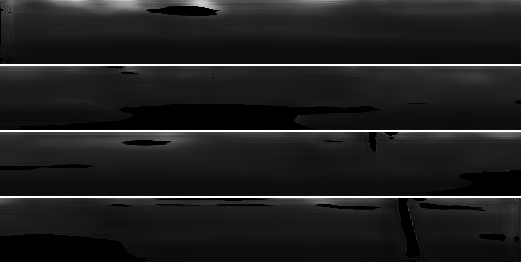
\includegraphics[keepaspectratio, width=\linewidth]{img/gta2valeo_depthgansr.png} & 
\includegraphics[keepaspectratio, width=\linewidth]{img/gta2valeo_intengansr.png} & 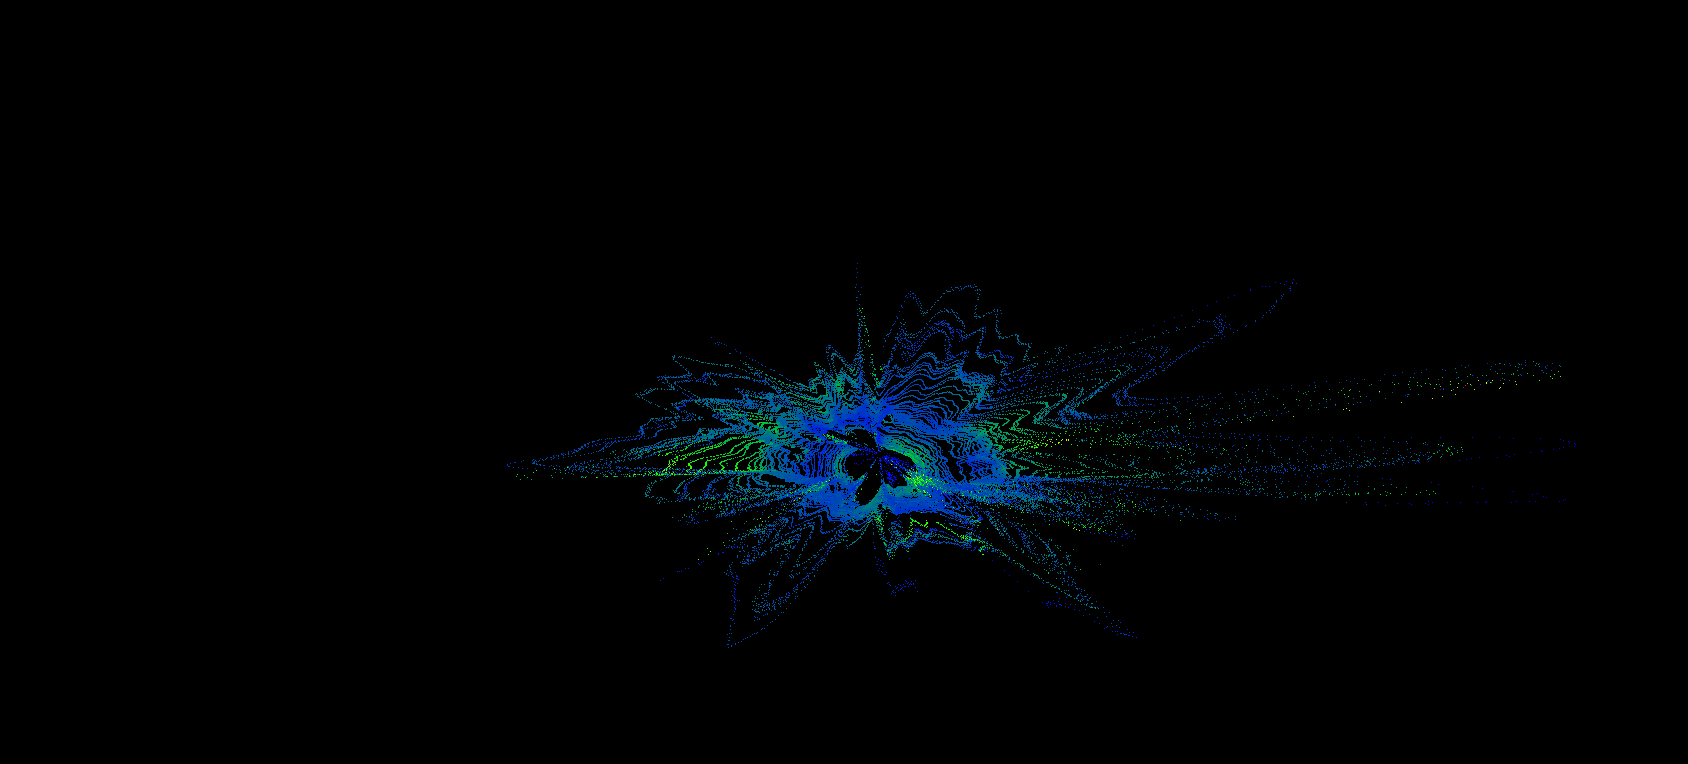
\includegraphics[keepaspectratio, width=\linewidth]{img/gta2valeo_pclgansr.png} \\
LSGAN\linebreak{}No Self-reg & 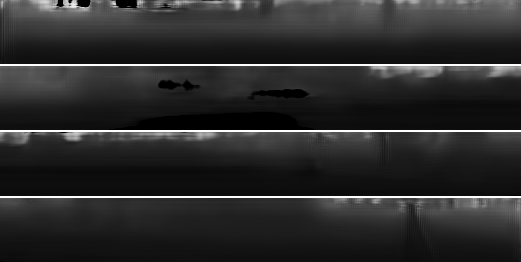
\includegraphics[keepaspectratio, width=\linewidth]{img/gta2valeo_depthlsgannosr.png} & 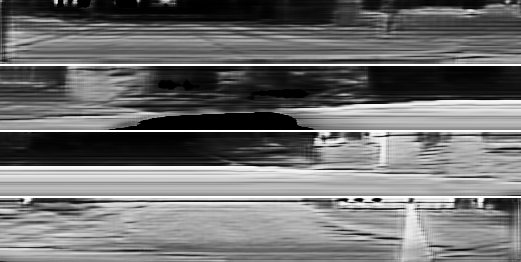
\includegraphics[keepaspectratio, width=\linewidth]{img/gta2valeo_intenlsgannosr.png} & 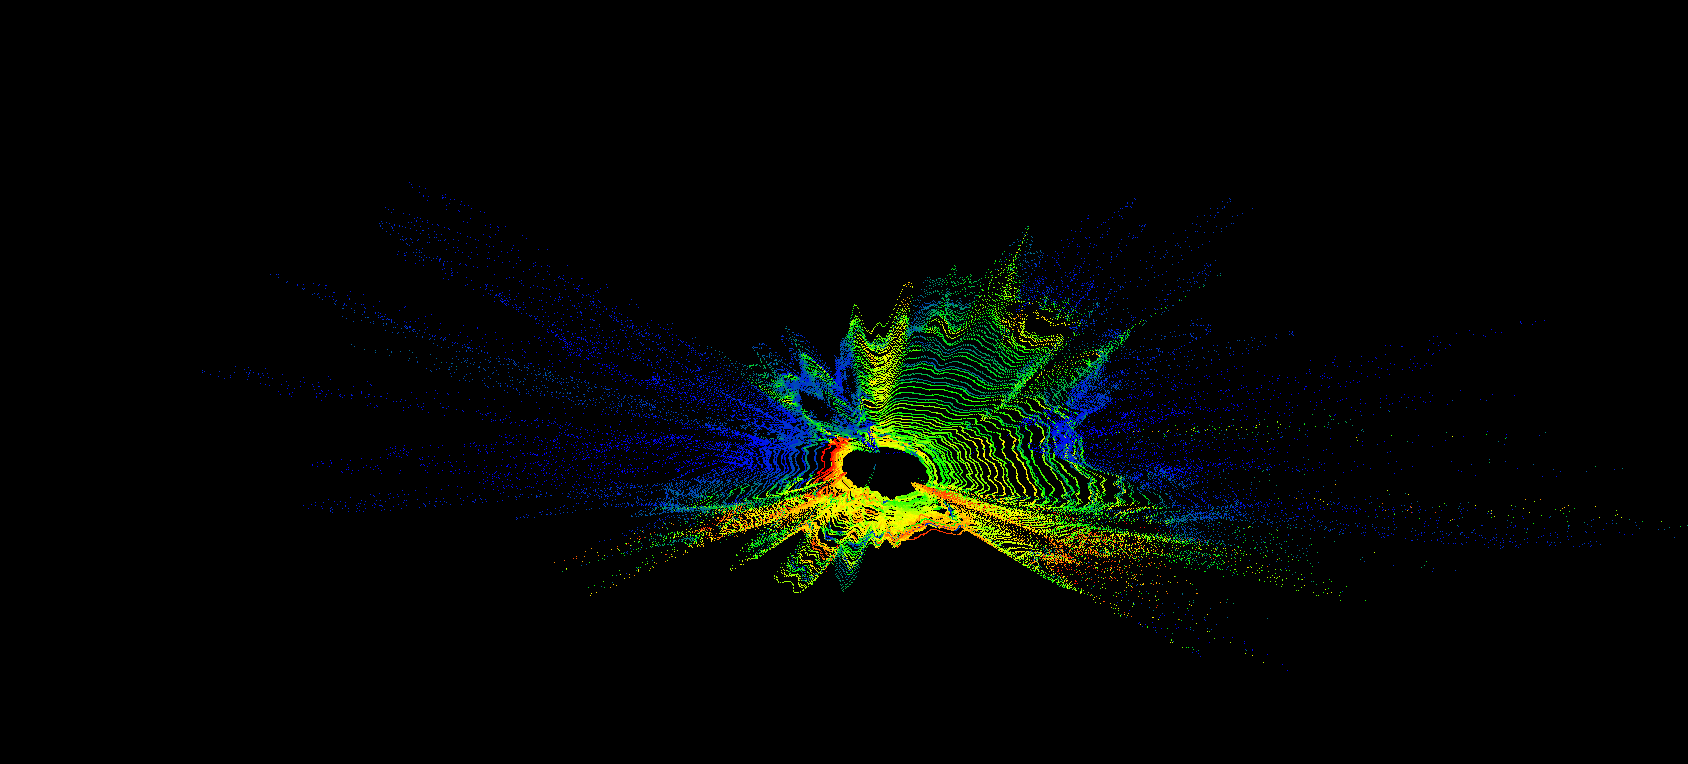
\includegraphics[keepaspectratio, width=\linewidth]{img/gta2valeo_pcllsgannosr.png} \\
LSGAN\linebreak{}Self-reg & 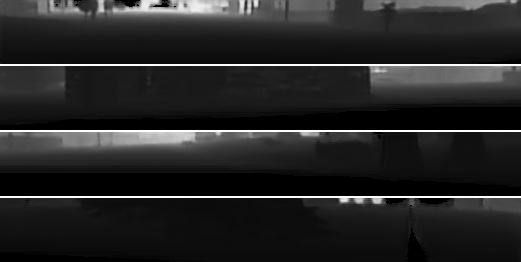
\includegraphics[keepaspectratio, width=\linewidth]{img/gta2valeo_depthlsgansr.png} & 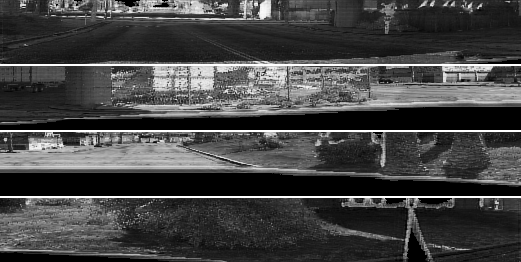
\includegraphics[keepaspectratio, width=\linewidth]{img/gta2valeo_intenlsgansr.png} & 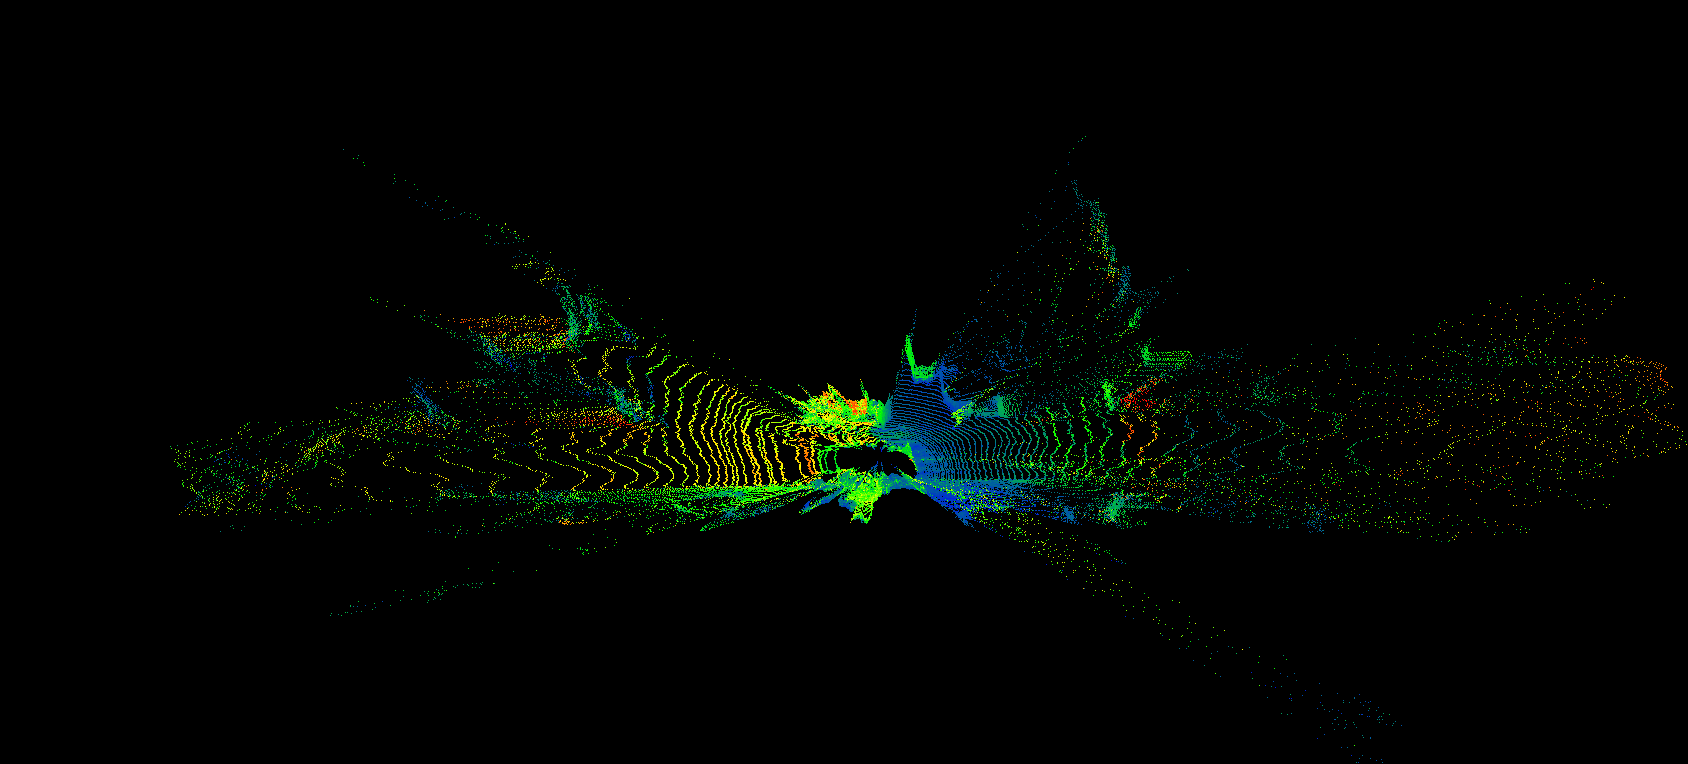
\includegraphics[keepaspectratio, width=\linewidth]{img/gta2valeo_pcllsgansr.png} \\
WGAN-GP\linebreak{}No Self-reg & 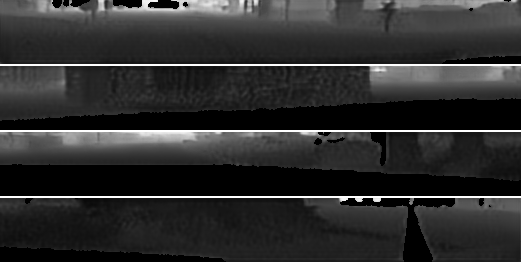
\includegraphics[keepaspectratio, width=\linewidth]{img/gta2valeo_depthwgannosr.png} & 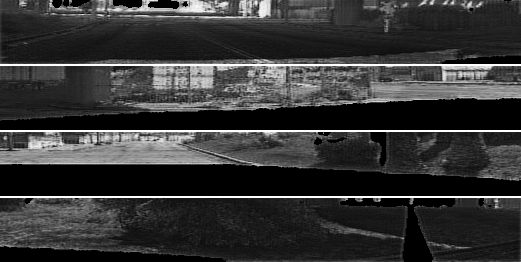
\includegraphics[keepaspectratio, width=\linewidth]{img/gta2valeo_intenwgannosr.png} & 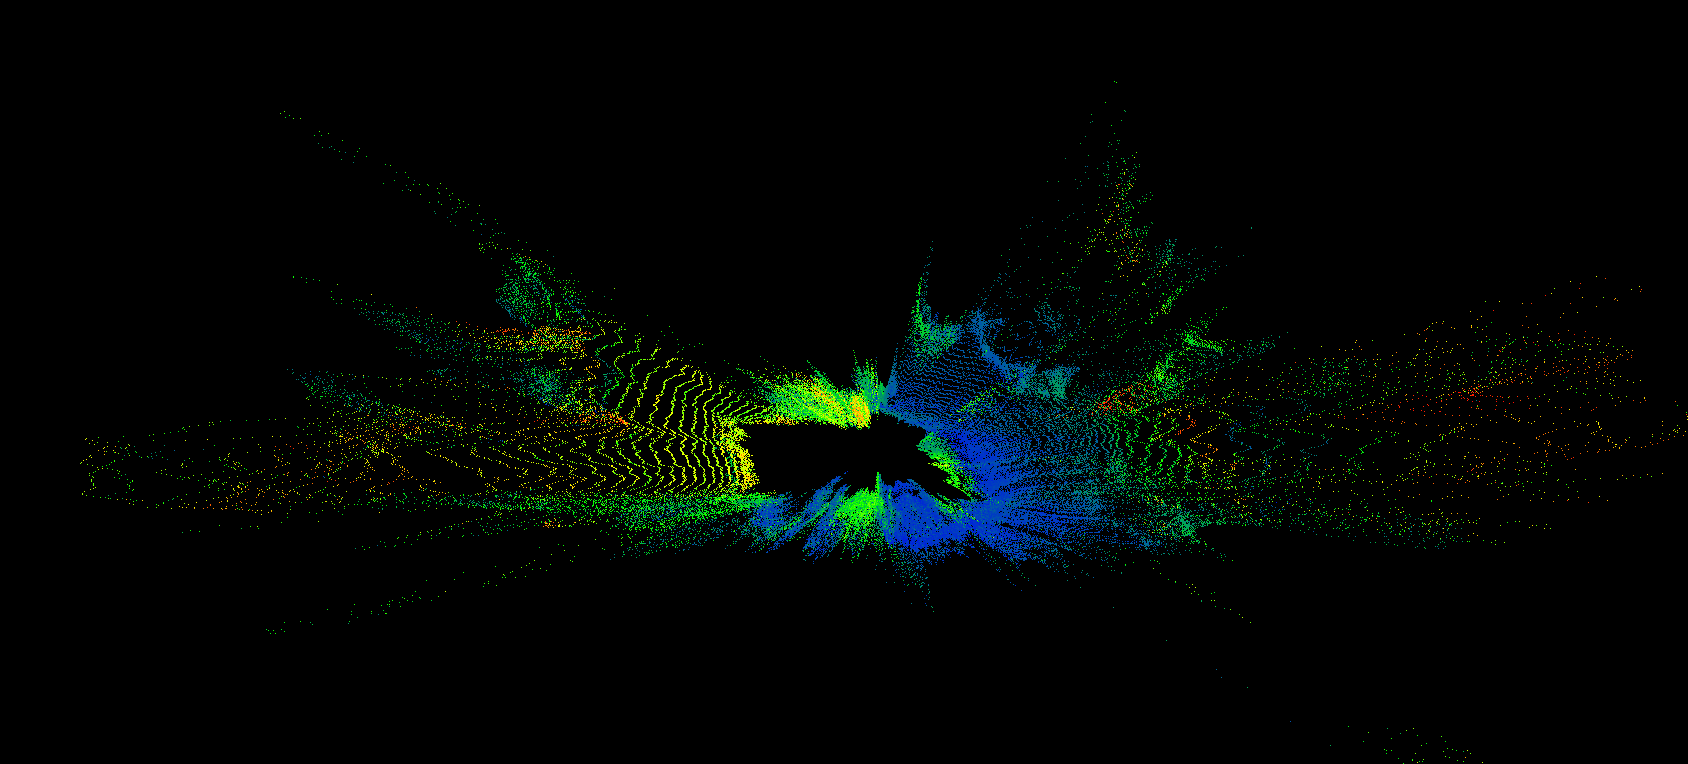
\includegraphics[keepaspectratio, width=\linewidth]{img/gta2valeo_pclwgannosr.png} \\
WGAN-GP\linebreak{}Self-reg & 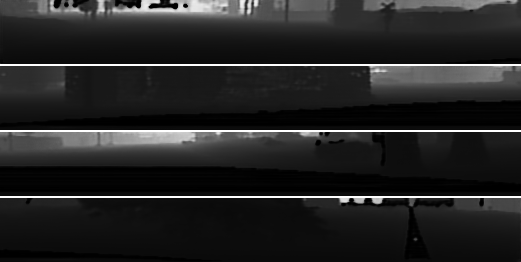
\includegraphics[keepaspectratio, width=\linewidth]{img/gta2valeo_depthwgansr.png} & 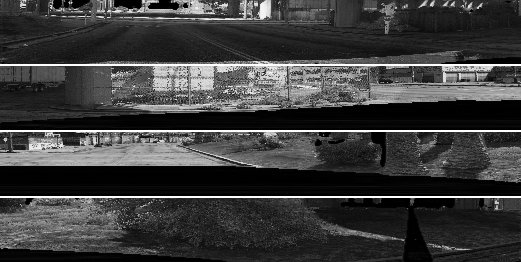
\includegraphics[keepaspectratio, width=\linewidth]{img/gta2valeo_intenwgansr.png} & 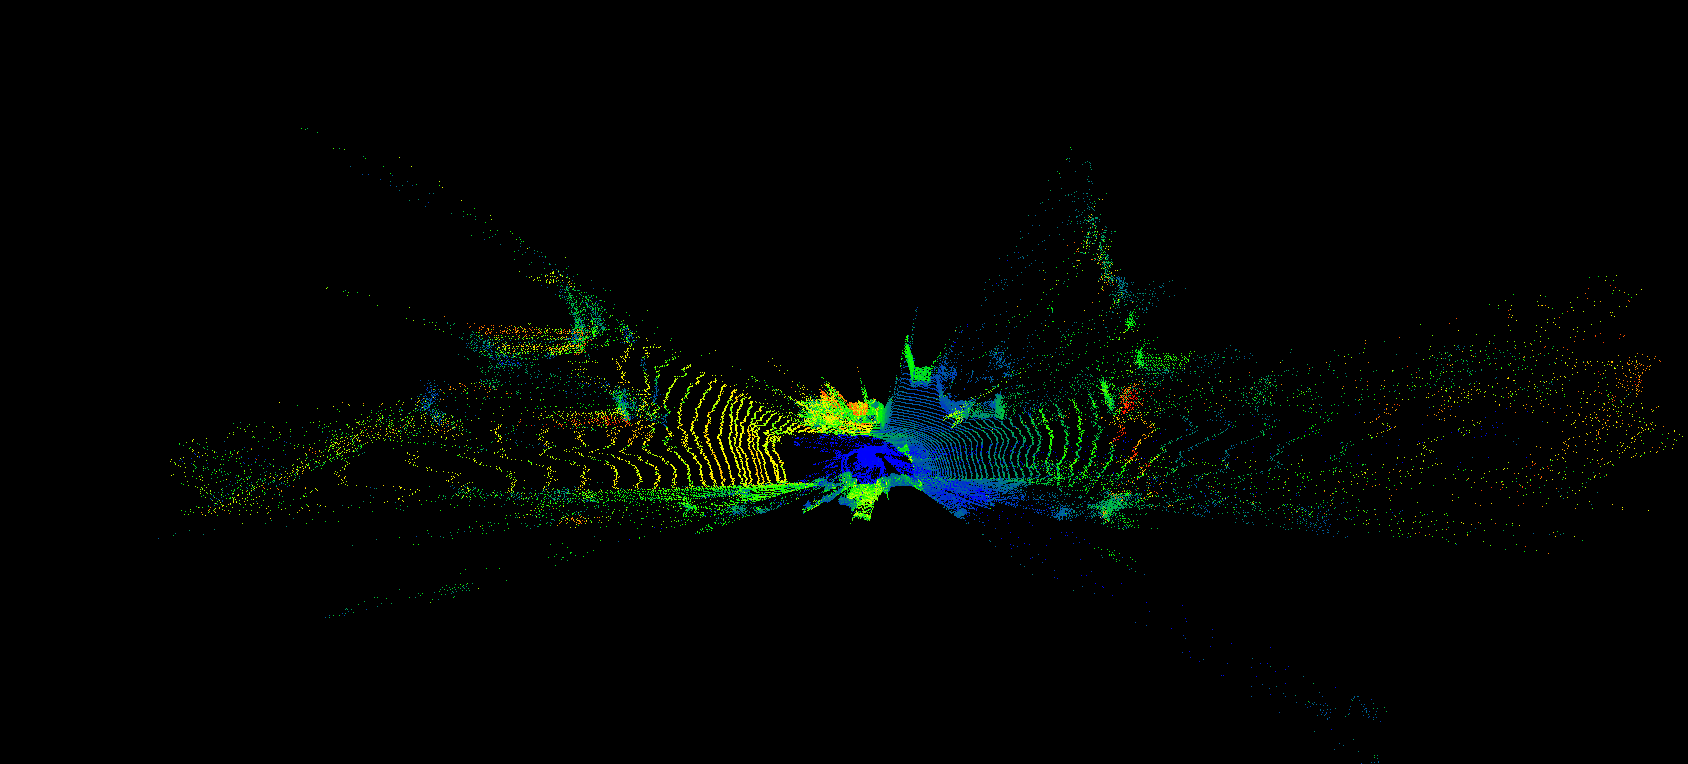
\includegraphics[keepaspectratio, width=\linewidth]{img/gta2valeo_pclwgansr.png} \\
\end{tabular}
\centering
\caption{Comparison of different GAN variants used in CycleGAN, GTA to Valeo}
\label{evalcmpg2v}
\end{figure}

\begin{figure}
\begin{tabular}{L|III}
 & \textbf{Depth} & \textbf{Intensity} & \textbf{Point cloud} \\
Original & 
\includegraphics[keepaspectratio, width=\linewidth]{img/gta2valeo_depthorigpart.png} & 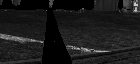
\includegraphics[keepaspectratio, width=\linewidth]{img/gta2valeo_intenorigpart.png} & 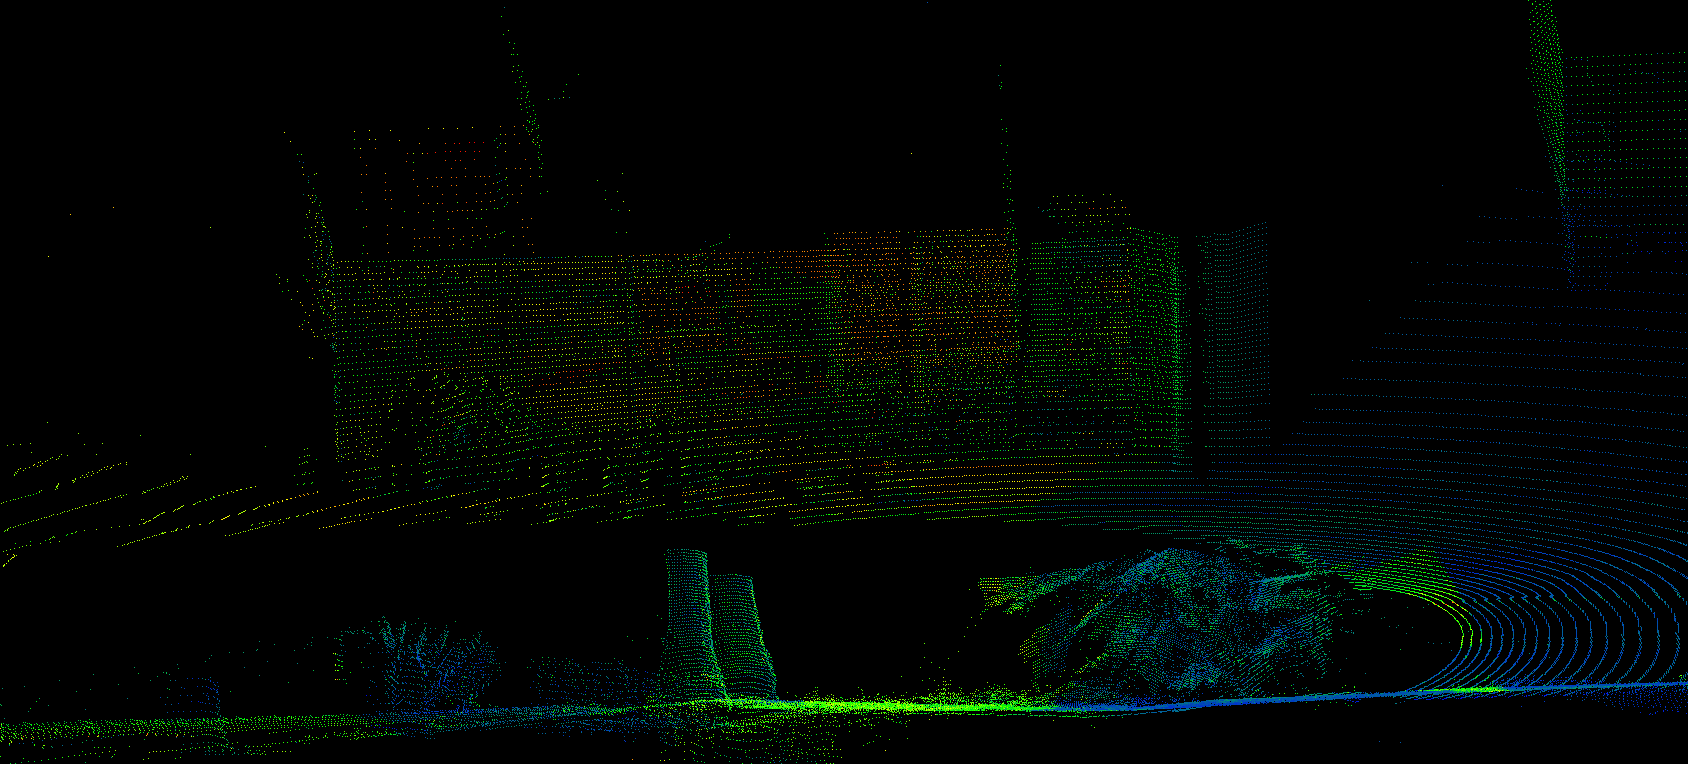
\includegraphics[keepaspectratio, width=\linewidth]{img/gta2valeo_pclorigpart.png} \\
GAN\linebreak{}No Self-reg & 
\includegraphics[keepaspectratio, width=\linewidth]{img/gta2valeo_depthgannosrpart.png} & 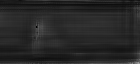
\includegraphics[keepaspectratio, width=\linewidth]{img/gta2valeo_intengannosrpart.png} & 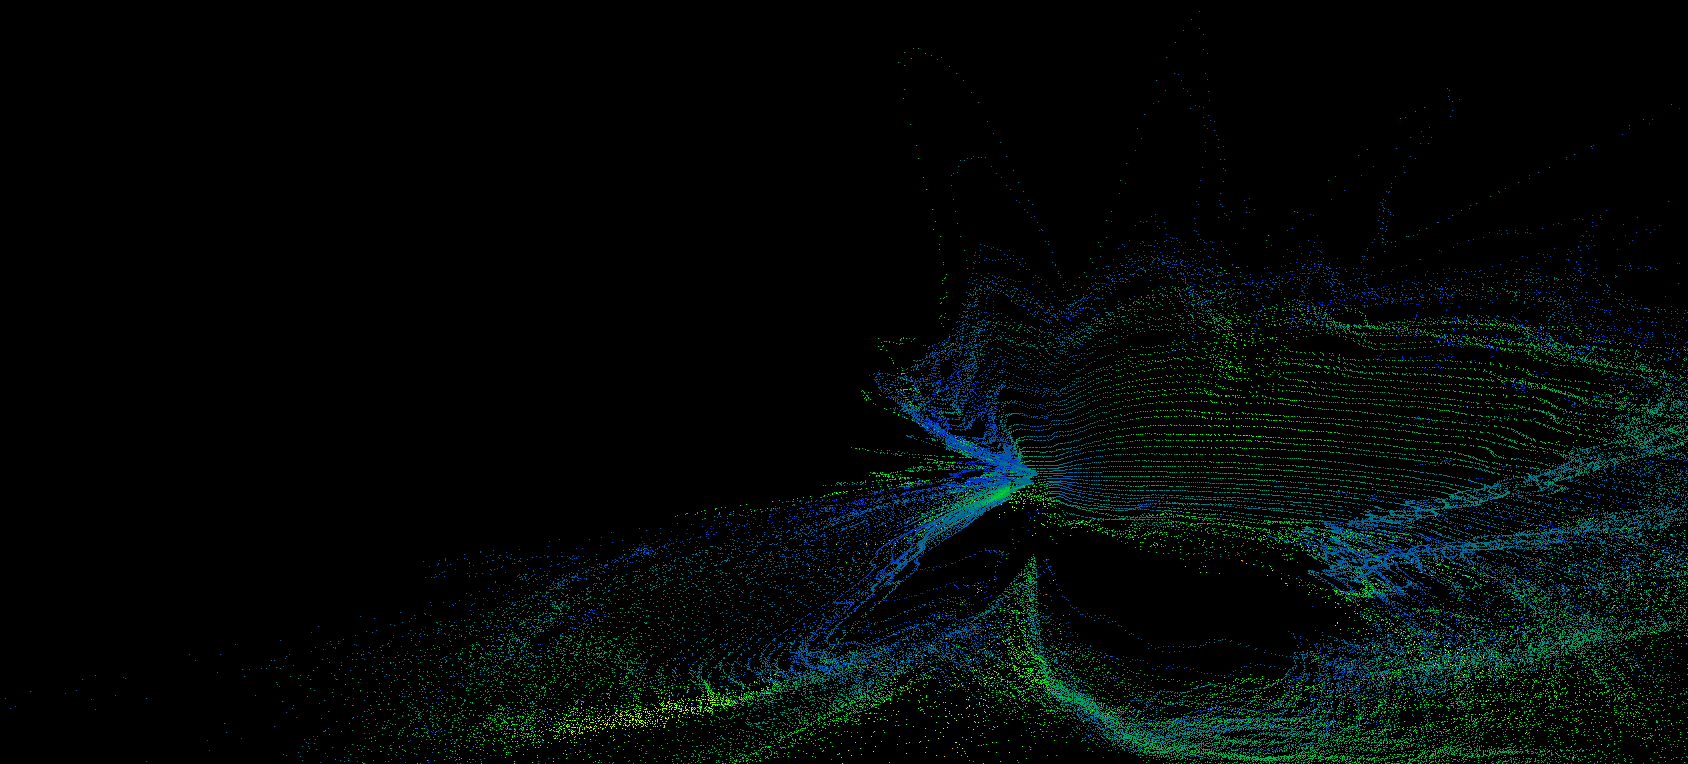
\includegraphics[keepaspectratio, width=\linewidth]{img/gta2valeo_pclgannosrpart.png} \\
GAN\linebreak{}Self-reg & 
\includegraphics[keepaspectratio, width=\linewidth]{img/gta2valeo_depthgansrpart.png} & 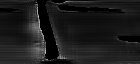
\includegraphics[keepaspectratio, width=\linewidth]{img/gta2valeo_intengansrpart.png} & 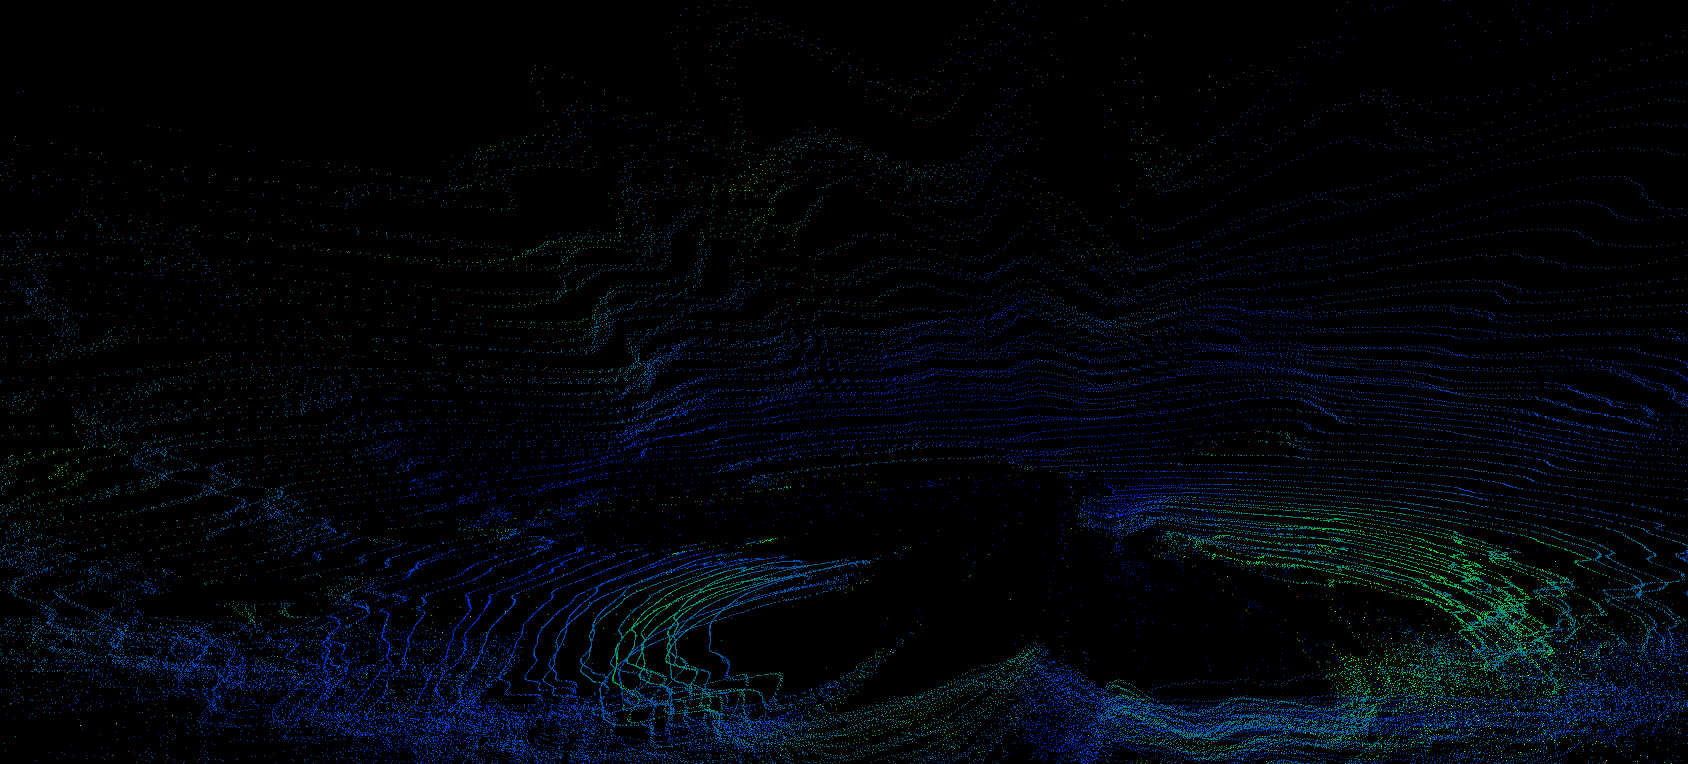
\includegraphics[keepaspectratio, width=\linewidth]{img/gta2valeo_pclgansrpart.png} \\
LSGAN\linebreak{}No Self-reg & 
\includegraphics[keepaspectratio, width=\linewidth]{img/gta2valeo_depthlsgannosrpart.png} & 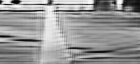
\includegraphics[keepaspectratio, width=\linewidth]{img/gta2valeo_intenlsgannosrpart.png} & 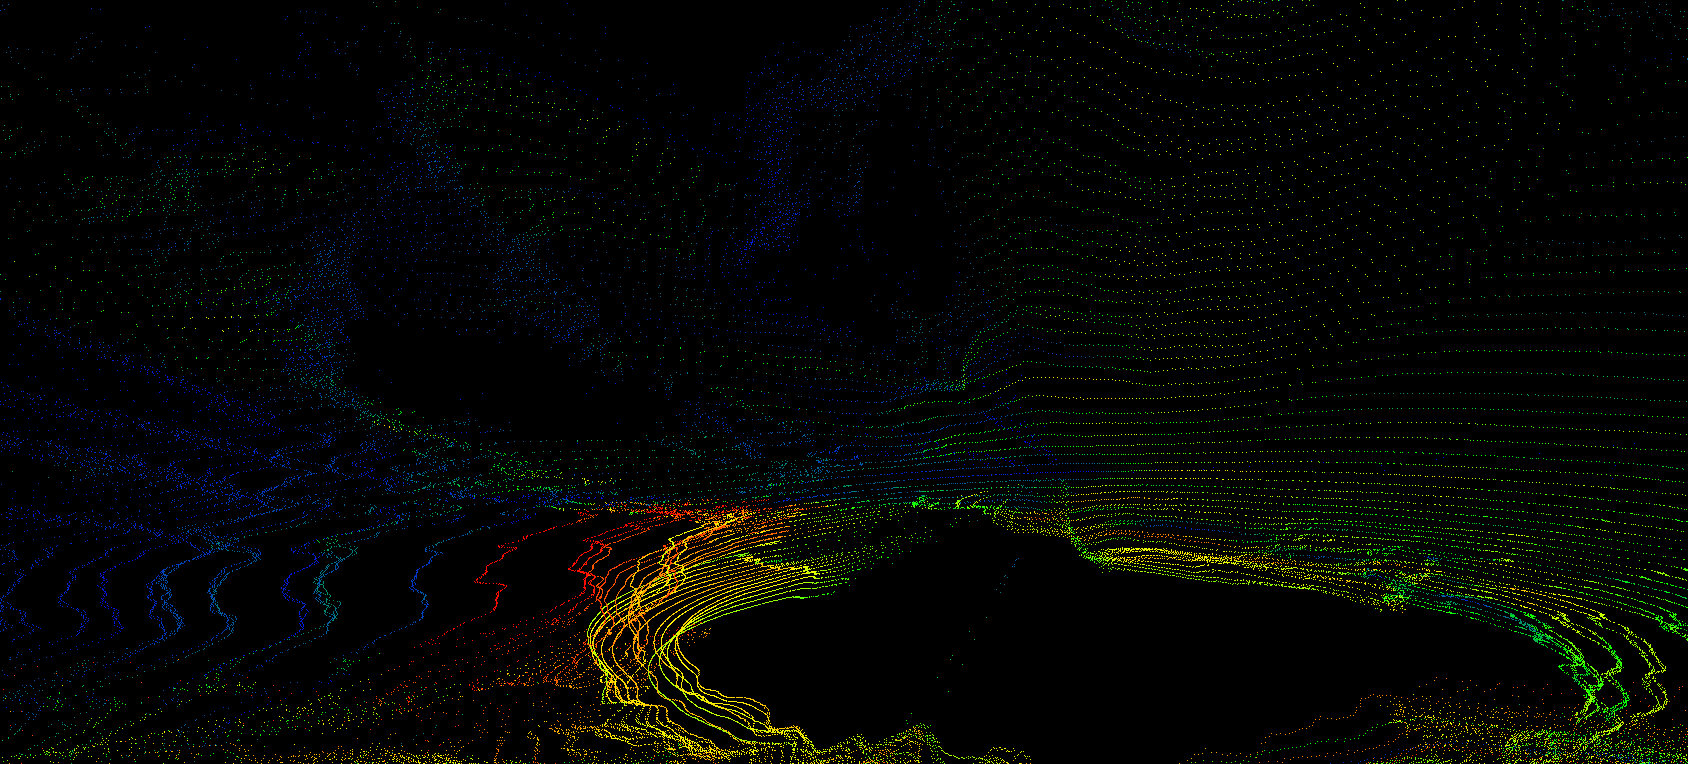
\includegraphics[keepaspectratio, width=\linewidth]{img/gta2valeo_pcllsgannosrpart.png} \\
LSGAN\linebreak{}Self-reg & 
\includegraphics[keepaspectratio, width=\linewidth]{img/gta2valeo_depthlsgansrpart.png} & 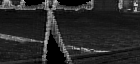
\includegraphics[keepaspectratio, width=\linewidth]{img/gta2valeo_intenlsgansrpart.png} & 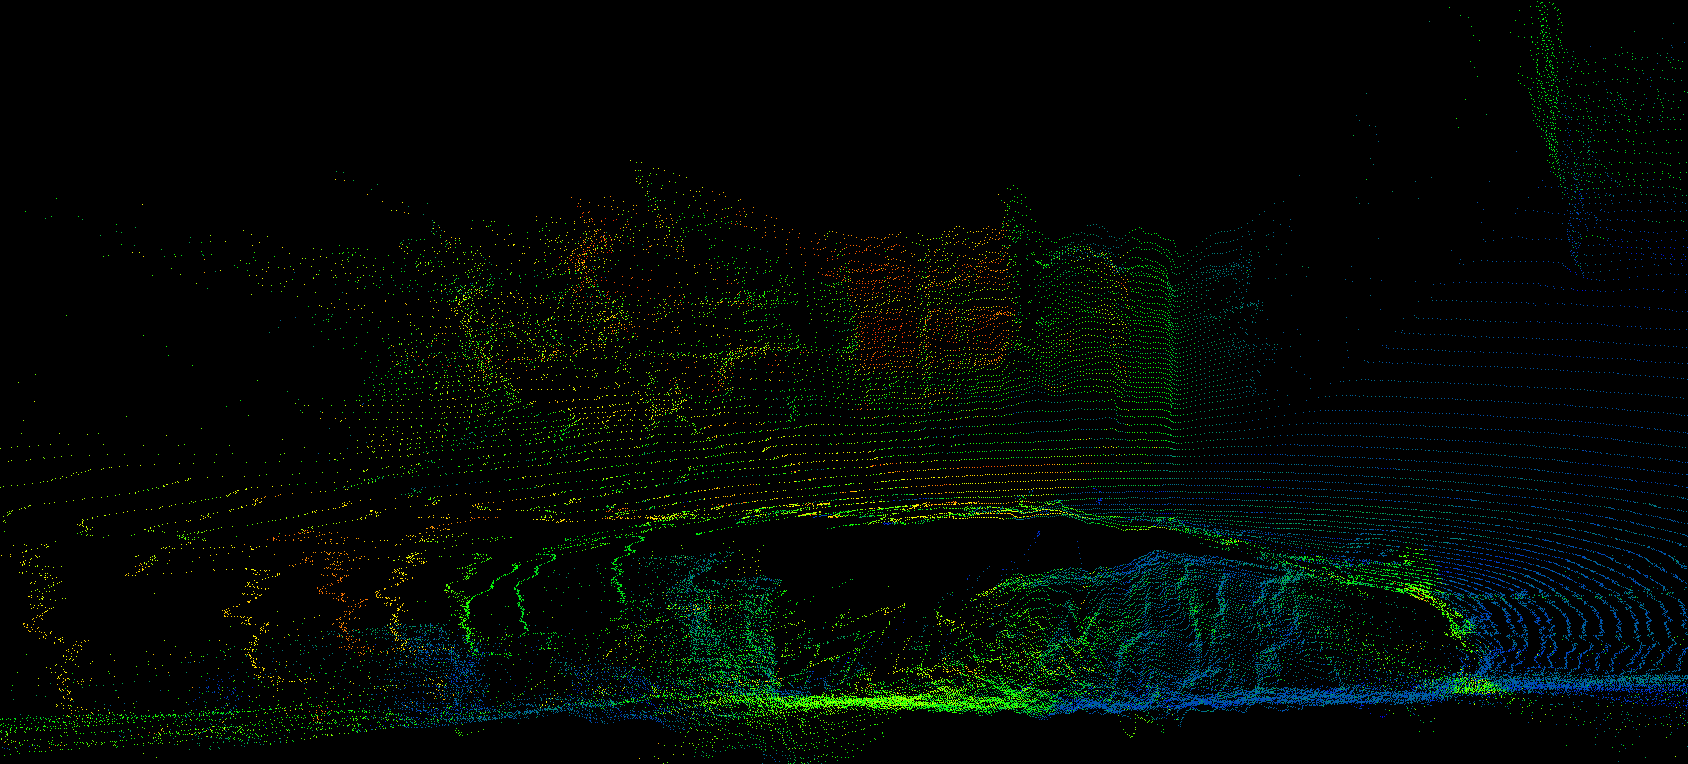
\includegraphics[keepaspectratio, width=\linewidth]{img/gta2valeo_pcllsgansrpart.png} \\
WGAN-GP\linebreak{}No Self-reg & 
\includegraphics[keepaspectratio, width=\linewidth]{img/gta2valeo_depthwgannosrpart.png} & 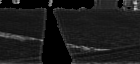
\includegraphics[keepaspectratio, width=\linewidth]{img/gta2valeo_intenwgannosrpart.png} & 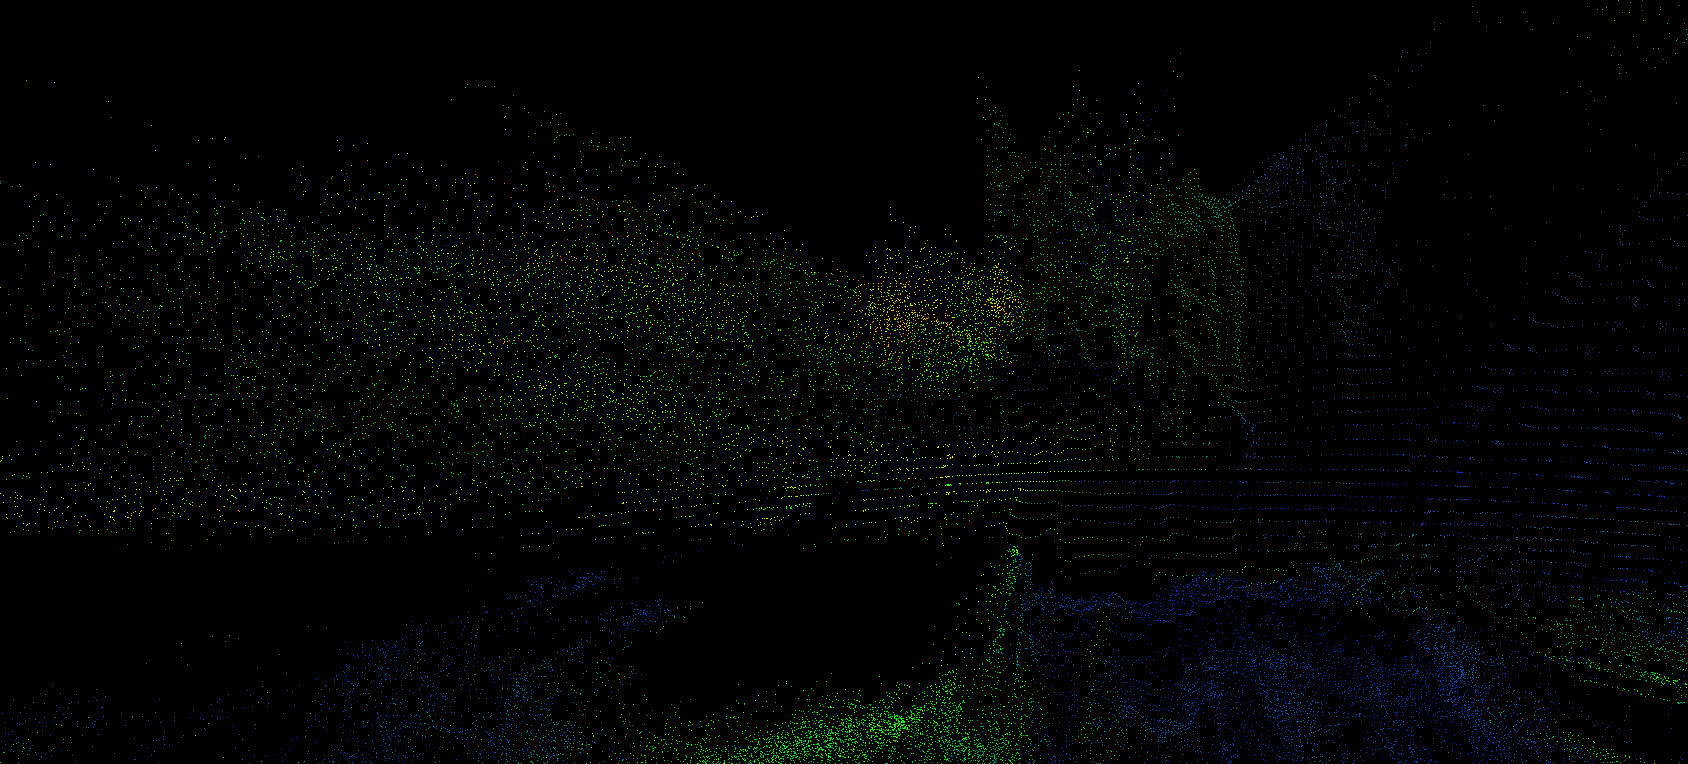
\includegraphics[keepaspectratio, width=\linewidth]{img/gta2valeo_pclwgannosrpart.png} \\
WGAN-GP\linebreak{}Self-reg & 
\includegraphics[keepaspectratio, width=\linewidth]{img/gta2valeo_depthwgansrpart.png} & \includegraphics[keepaspectratio, width=\linewidth]{img/gta2valeo_intenwgansrpart.png} & \includegraphics[keepaspectratio, width=\linewidth]{img/gta2valeo_pclwgansrpart.png} \\
\end{tabular}
\centering
\caption[Comparison of different GAN variants used in CycleGAN, GTA to Valeo, cutout]{Comparison of different GAN variants used in CycleGAN, in a GTA to Valeo direction. Only a small part of the image is shown for better clarity.}
\label{evalcmpg2vcutout}
\end{figure}

\begin{figure}
\begin{tabular}{L|III}
 & \textbf{Depth} & \textbf{Intensity} & \textbf{Point cloud} \\
Original & \includegraphics[keepaspectratio, width=\linewidth]{img/valeo2gta_depthorig.png} & \includegraphics[keepaspectratio, width=\linewidth]{img/valeo2gta_intenorig.png} & \includegraphics[keepaspectratio, width=\linewidth]{img/valeo2gta_pclorig.png} \\
GAN\linebreak{}No Self-reg & \includegraphics[keepaspectratio, width=\linewidth]{img/valeo2gta_depthgannosr.png} & \includegraphics[keepaspectratio, width=\linewidth]{img/valeo2gta_intengannosr.png} & \includegraphics[keepaspectratio, width=\linewidth]{img/valeo2gta_pclgannosr.png} \\
GAN\linebreak{}Self-reg & \includegraphics[keepaspectratio, width=\linewidth]{img/valeo2gta_depthgansr.png} & \includegraphics[keepaspectratio, width=\linewidth]{img/valeo2gta_intengansr.png} & \includegraphics[keepaspectratio, width=\linewidth]{img/valeo2gta_pclgansr.png} \\
LSGAN\linebreak{}No Self-reg & \includegraphics[keepaspectratio, width=\linewidth]{img/valeo2gta_depthlsgannosr.png} & \includegraphics[keepaspectratio, width=\linewidth]{img/valeo2gta_intenlsgannosr.png} & \includegraphics[keepaspectratio, width=\linewidth]{img/valeo2gta_pcllsgannosr.png} \\
LSGAN\linebreak{}Self-reg & \includegraphics[keepaspectratio, width=\linewidth]{img/valeo2gta_depthlsgansr.png} & \includegraphics[keepaspectratio, width=\linewidth]{img/valeo2gta_intenlsgansr.png} & \includegraphics[keepaspectratio, width=\linewidth]{img/valeo2gta_pcllsgansr.png} \\
WGAN-GP\linebreak{}No Self-reg & \includegraphics[keepaspectratio, width=\linewidth]{img/valeo2gta_depthwgannosr.png} & \includegraphics[keepaspectratio, width=\linewidth]{img/valeo2gta_intenwgannosr.png} & \includegraphics[keepaspectratio, width=\linewidth]{img/valeo2gta_pclwgannosr.png} \\
WGAN-GP\linebreak{}Self-reg & \includegraphics[keepaspectratio, width=\linewidth]{img/valeo2gta_depthwgansr.png} & \includegraphics[keepaspectratio, width=\linewidth]{img/valeo2gta_intenwgansr.png} & \includegraphics[keepaspectratio, width=\linewidth]{img/valeo2gta_pclwgansr.png} \\
\end{tabular}
\centering
\caption{Comparison of different GAN variants used in CycleGAN, Valeo to GTA}
\label{evalcmpv2g}
\end{figure}

\begin{figure}
\begin{tabular}{L|III}
 & \textbf{Depth} & \textbf{Intensity} & \textbf{Point cloud} \\
Original & \includegraphics[keepaspectratio, width=\linewidth]{img/valeo2gta_depthorigpart.png} & \includegraphics[keepaspectratio, width=\linewidth]{img/valeo2gta_intenorigpart.png} & \includegraphics[keepaspectratio, width=\linewidth]{img/valeo2gta_pclorigpart.png} \\
GAN\linebreak{}No Self-reg & \includegraphics[keepaspectratio, width=\linewidth]{img/valeo2gta_depthgannosrpart.png} & \includegraphics[keepaspectratio, width=\linewidth]{img/valeo2gta_intengannosrpart.png} & \includegraphics[keepaspectratio, width=\linewidth]{img/valeo2gta_pclgannosrpart.png} \\
GAN\linebreak{}Self-reg & \includegraphics[keepaspectratio, width=\linewidth]{img/valeo2gta_depthgansrpart.png} & \includegraphics[keepaspectratio, width=\linewidth]{img/valeo2gta_intengansrpart.png} & \includegraphics[keepaspectratio, width=\linewidth]{img/valeo2gta_pclgansrpart.png} \\
LSGAN\linebreak{}No Self-reg & \includegraphics[keepaspectratio, width=\linewidth]{img/valeo2gta_depthlsgannosrpart.png} & \includegraphics[keepaspectratio, width=\linewidth]{img/valeo2gta_intenlsgannosrpart.png} & \includegraphics[keepaspectratio, width=\linewidth]{img/valeo2gta_pcllsgannosrpart.png} \\
LSGAN\linebreak{}Self-reg & \includegraphics[keepaspectratio, width=\linewidth]{img/valeo2gta_depthlsgansrpart.png} & \includegraphics[keepaspectratio, width=\linewidth]{img/valeo2gta_intenlsgansrpart.png} & \includegraphics[keepaspectratio, width=\linewidth]{img/valeo2gta_pcllsgansrpart.png} \\
WGAN-GP\linebreak{}No Self-reg & \includegraphics[keepaspectratio, width=\linewidth]{img/valeo2gta_depthwgannosrpart.png} & \includegraphics[keepaspectratio, width=\linewidth]{img/valeo2gta_intenwgannosrpart.png} & \includegraphics[keepaspectratio, width=\linewidth]{img/valeo2gta_pclwgannosrpart.png} \\
WGAN-GP\linebreak{}Self-reg & \includegraphics[keepaspectratio, width=\linewidth]{img/valeo2gta_depthwgansrpart.png} & \includegraphics[keepaspectratio, width=\linewidth]{img/valeo2gta_intenwgansrpart.png} & \includegraphics[keepaspectratio, width=\linewidth]{img/valeo2gta_pclwgansrpart.png} \\
\end{tabular}
\centering
\caption[Comparison of different GAN variants used in CycleGAN, Valeo to GTA, cutout]{Comparison of different GAN variants used in CycleGAN, in a Valeo to GTA direction. Only a small part of the image is shown for better clarity.}
\label{evalcmpv2gcutout}
\end{figure}

\chapter{Conclusion}

\section{Discussion of the achieved results}

It is important to note, that there seems to be no universally accepted evaluation metric of realism. Most of today's generative networks are compared using Inception score~\cite{inception}, however, this is only suitable if one is generating actual images and not the depth image with completely different semantics. Another option researches often use is Amazon's Mechanical Turk, however this suffers from the limitation that it might not be clearly obvious how a ``real'' LiDAR-like image (or reconstructed point cloud) from a GTA or Valeo dataset should look like. To properly evaluate the results, whole pipeline using these refined artificial data is needed which was not in the scope of this thesis. Therefore we performed only qualitative analysis of the results showing the generated images.

If we look at the data shown in the figures \ref{evalcmpg2v} and \ref{evalcmpv2g}, we can safely say that the original GAN does not work in this setting regardless of the self regularization of the generators.

This seems to hold for LSGAN without self-regularization as well, however when self-regularization was added, LSGAN started to perform a lot better, preserving the important intensity information. However, it is safe to say that even without rigorous evaluation metric, WGAN-GP with self-regularization term was the winner. It seems to be able to maintain the important information and to introduce noise similar to the real world noise when transforming from the GTA dataset to Valeo dataset, as seen in the point cloud portion of the results.

The most important part of the results is the fact, that the generator of the WGAN-GP network with the self-regularization loss term is able to distinguish between the different objects in the scene and adds the noise in accordance with the expected noise induced by different objects. This can be visible at the figure \ref{carfigs}, where left figure is the original intensity of the car in the GTA data, right figure is the intensity from the refined intensity by WGAN-GP and center figure is the difference between the two figures scaled by 10. The difference is shown in such a way, that if there was no difference, the color has gray-scale value of 0.5 and if the color is lighter than 0.5, then the original intensity was higher than the converted intensity and vice-versa. As you can see, the car and surrounding road is still distinguishable even in the difference image indicating that the generated difference depends on the semantics of the object in the original image. If you look more closely, you can see that the intensity was {\em lowered} on the car which has reflective surface and {\em raised} on the road which is in accordance with the physical state of the world.

\begin{figure}
\subfloat[Original intensity on the car]{\includegraphics[keepaspectratio, width=0.3\linewidth]{img/carorig.png}}
\hfil
\subfloat[Difference of intensities]{\includegraphics[keepaspectratio, width=0.3\linewidth]{img/cardiff.png}}
\hfil
\subfloat[Refined intensity on the car]{\includegraphics[keepaspectratio, width=0.3\linewidth]{img/carconv.png}}
\caption{Comparison of LiDAR intensities on the car}
\label{carfigs}
\end{figure}

\section{Future work}

In the future we would like to develop a sensible metric for generating depth data. This can be seen as the biggest shortcoming of this thesis. It will be also beneficial to leverage more information from the data in order to be able to create more accurate models of the depth sensors. The most beneficial would be to use RGB data with the LiDAR data simultaneously, however this was not possible due to the missing calibrated RGB images in the Valeo dataset.

It might be interesting to explore the idea of asymmetric CycleGAN in which the generators' structures as well as the input and output shapes differ. This use-case can be potentially very interesting as it can lead to using more information from one dataset if available.

\section{Conclusion}

We showed that the generative modeling of LiDAR-like data is feasible in the CycleGAN setting. This is an important result since as far as we know it was never tried before. The results indicate that it is necessary to be extremely careful about used loss functions and underlying generative models used in the CycleGAN. We believe that if more detailed data (namely RGB images corresponding to the LiDAR scans) were available to the training pipeline, achieved results would be even more convincing.


\newpage
\bibliographystyle{unsrtnat}
\bibliography{jasek}


\end{document}
